\documentclass[a4paper, 11pt, oneside, polutonikogreek, german]{article}
\usepackage{kmath, kerkis}
\usepackage[T1]{fontenc}

% Load encoding definitions (after font package)

\usepackage{textalpha}
\usepackage{listings}
\lstset{basicstyle=\ttfamily}

\usepackage[dvipsnames]{xcolor}
\usepackage{eso-pic,graphicx}
\usepackage[top=65mm, bottom=82mm, outer=49mm, inner=49mm]{geometry}
\setlength{\columnsep}{90pt}

% Babel package:
\usepackage[greek]{babel}

% With XeTeX$\$LuaTeX, load fontspec after babel to use Unicode
% fonts for Latin script and LGR for Greek:
\ifdefined\luatexversion \usepackage{fontspec}\fi
\ifdefined\XeTeXrevision \usepackage{fontspec}\fi

% "Lipsiakos" italic font `cbleipzig`:
\newcommand*{\lishape}{\fontencoding{LGR}\fontfamily{cmr}%
		       \fontshape{li}\selectfont}
\DeclareTextFontCommand{\textli}{\lishape}

\usepackage{setspace}
\onehalfspacing

\usepackage{booktabs}
\setlength{\emergencystretch}{5pt}
\usepackage{fancyhdr}
\usepackage{microtype}

% change color of text, example replace all \color{Goldenrod} with \color{lightgray}

\makeatletter % change only the display of \thepage, but not \thepage itself:
\patchcmd{\ps@plain}{\thepage}{\bfseries\large\color{Cerulean}{\thepage}}{}{}
\makeatother

\color{Cerulean}

\begin{document}
\AddToShipoutPictureBG{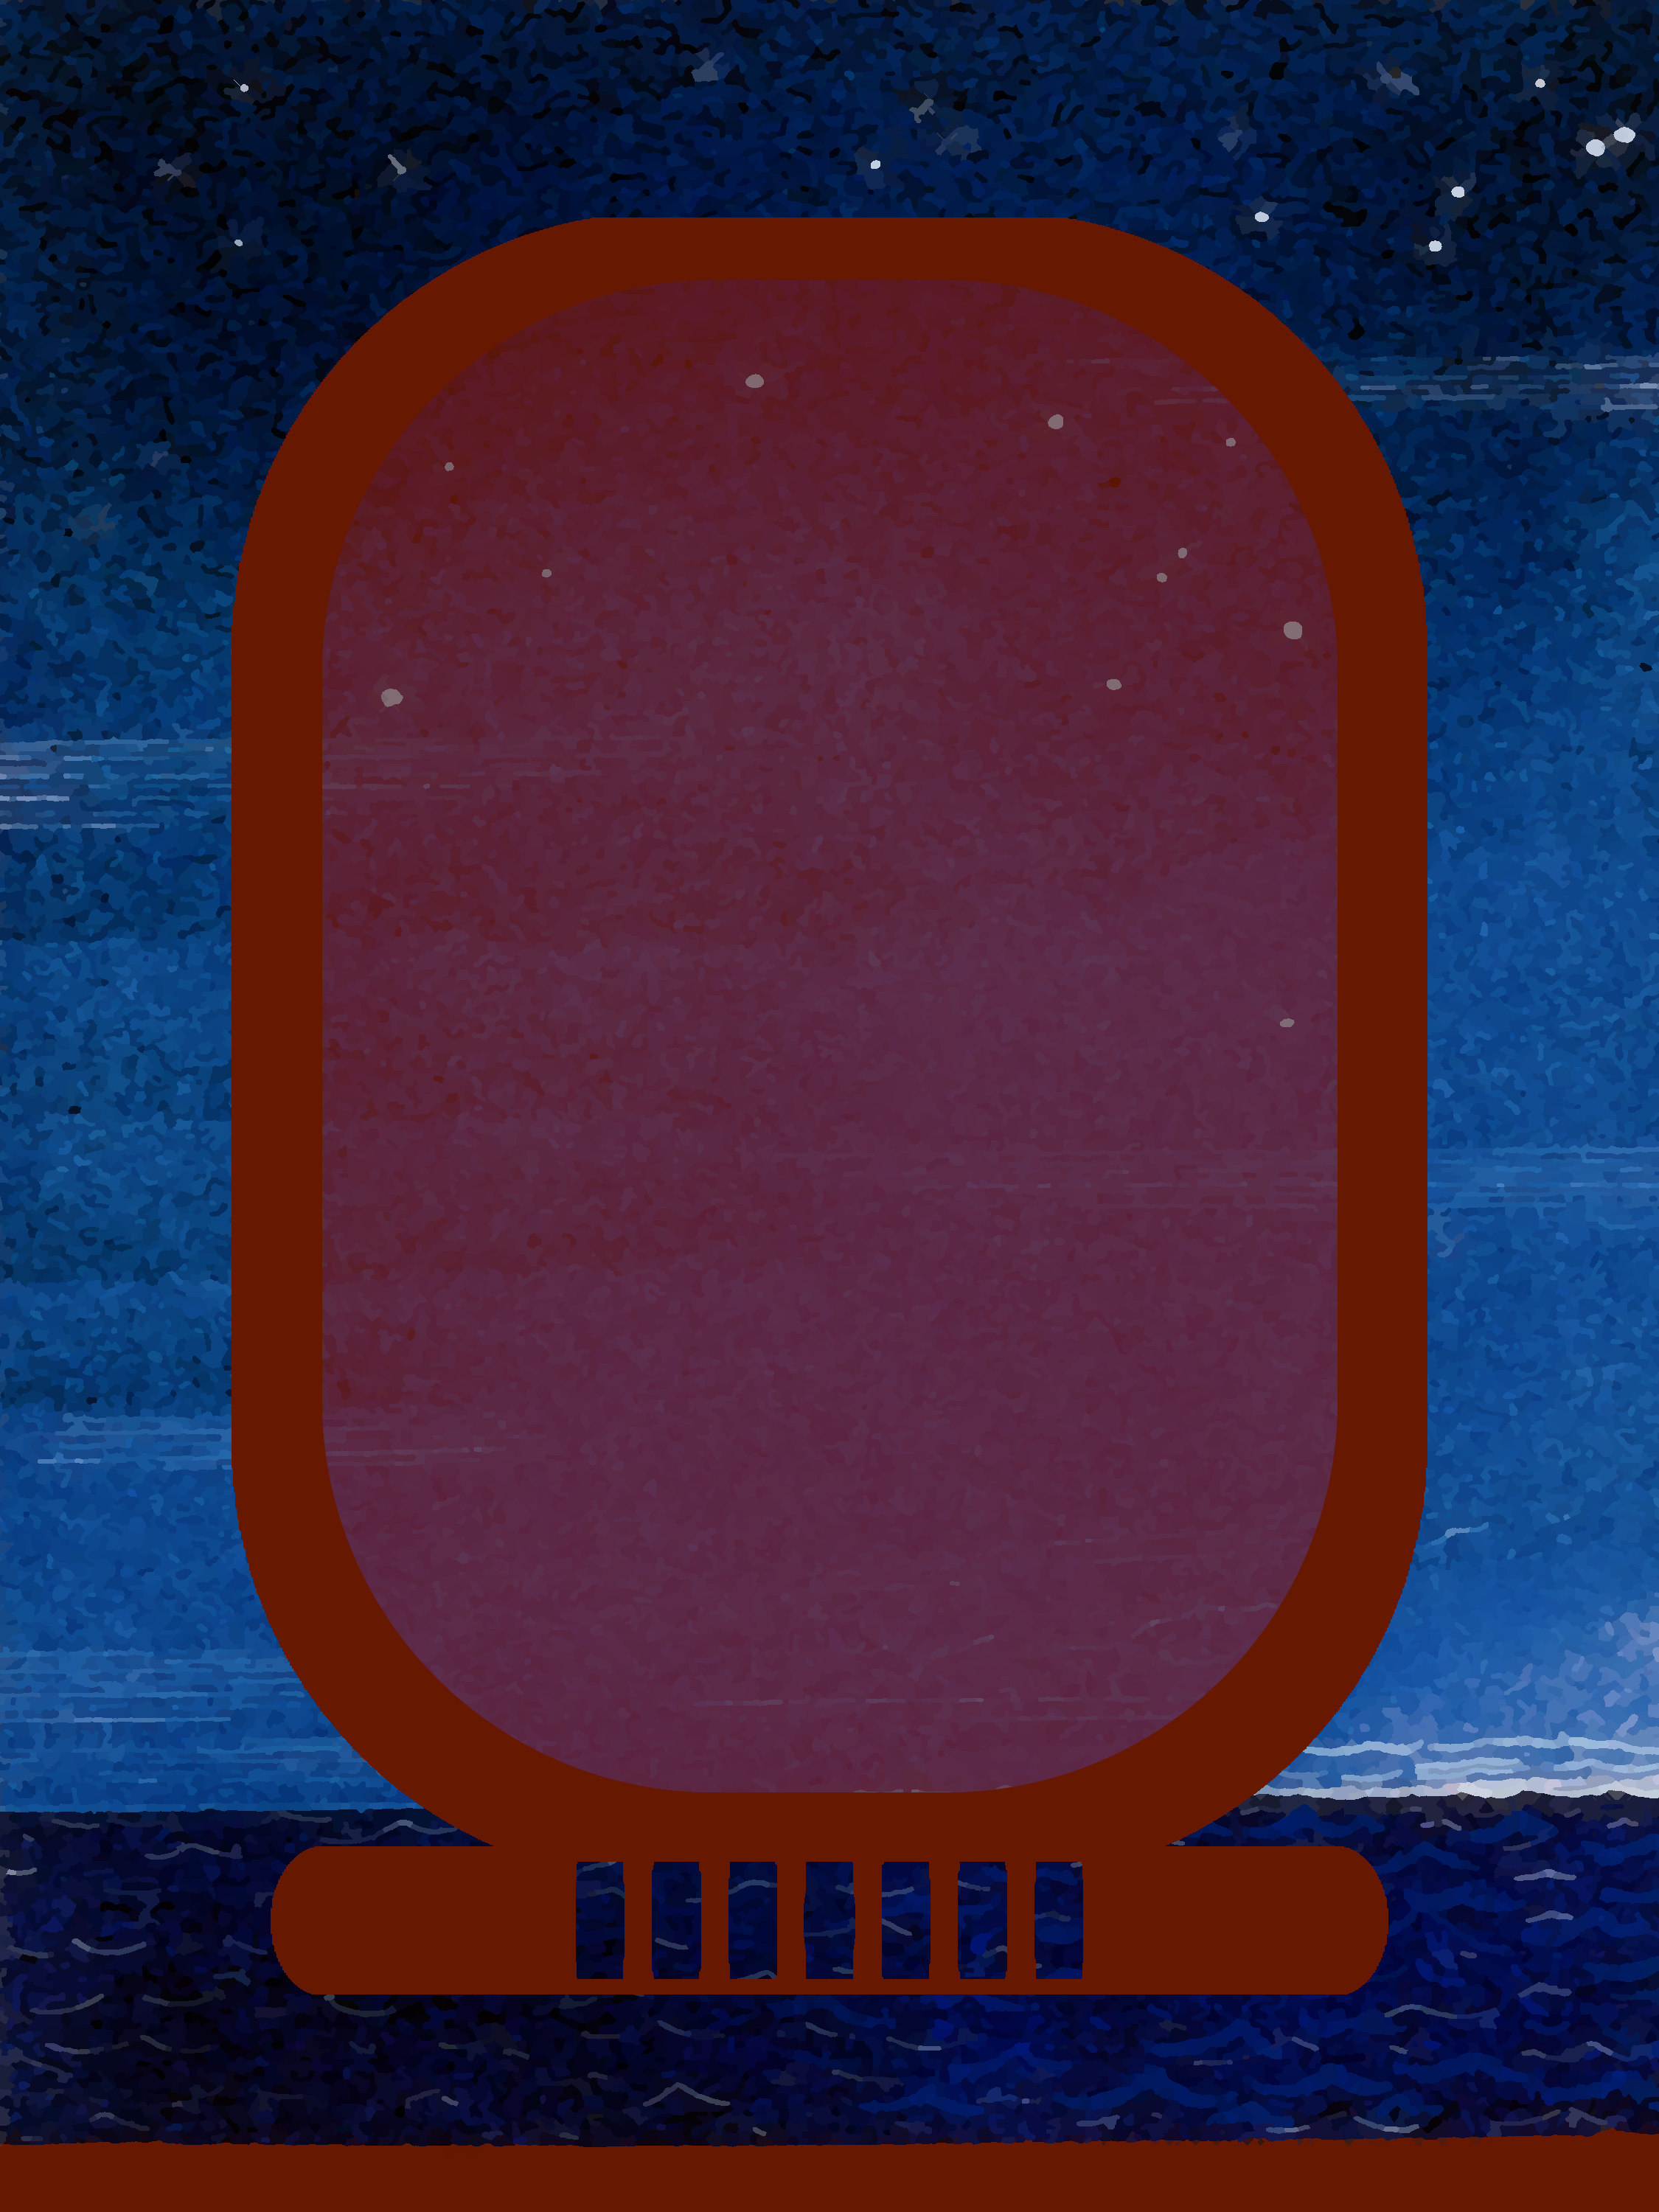
\includegraphics[width=\paperwidth,height=\paperheight]{greek1.jpeg}}
\begin{titlepage} % Suppresses headers and footers on the title page
	\centering % Centre everything on the title page
	%\scshape % Use small caps for all text on the title page

	%------------------------------------------------
	%	Title
	%------------------------------------------------

	\rule{\textwidth}{1.6pt}\vspace*{-\baselineskip}\vspace*{2pt} % Thick horizontal rule
	\rule{\textwidth}{0.4pt} % Thin horizontal rule
	
	\vspace{1\baselineskip} % Whitespace above the title
	
	{\scshape\Huge Αληθούς Ιστορίας}
	
	\vspace{1\baselineskip} % Whitespace above the title

	\rule{\textwidth}{0.4pt}\vspace*{-\baselineskip}\vspace{3.2pt} % Thin horizontal rule
	\rule{\textwidth}{1.6pt} % Thick horizontal rule
	
	\vspace{1\baselineskip} % Whitespace after the title block
	
	%------------------------------------------------
	%	Subtitle
	%------------------------------------------------
	
	{\scshape \Large Λουκιανός}
 
        \vspace{0.5\baselineskip}
	
	\vspace*{1\baselineskip} % Whitespace under the subtitle
	
        {\scshape \normalsize } % Subtitle or further description

	%------------------------------------------------
	%	Editor(s)
	%------------------------------------------------
        \vspace*{\fill}    

	\vspace{1\baselineskip}

	{\small\scshape 1852}
	
	{\small\scshape{Sumptibus et Typis B. G. Teubneri}}
	
	\vspace{0.5\baselineskip} % Whitespace after the title block

        \scshape Internet Archive Online Edition% Publication year
    
	{\scshape\small Creative Commons Αναφορά-Μη Εμπορική Χρήση 4.0} % Publisher
\end{titlepage}
\setlength{\parskip}{1mm plus1mm minus1mm}
\clearpage
\large
%\tableofcontents
%\clearpage
\begin{center}
\section{Λογος Πρωτος}
\end{center}
\paragraph{}
\textbf{1.} Ὥσπερ τοῖς ἀθλητικοῖς καὶ περὶ τὴν τῶν σωμάτων ἐπιμέλειαν ἠσκημένοις οὐ τῆς εὐεξίας μόνον οὐδὲ τῶν γυμνασίων φροντίς ἐστιν, ἀλλὰ καὶ τῆς κατὰ καιρὸν γινομένης ἀνέσεως --- μέρος γοῦν τῆς ἀσκήσεως τὸ μέγιστον αὐτὴν ὑπολαμβάνουσιν --- οὕτω δὴ καὶ τοῖς περὶ τοὺς λόγους ἐσπουδακόσιν ἡγοῦμαι προσήκειν μετὰ τὴν πολλὴν τῶν σπουδαιοτέρων ἀνάγνωσιν ἀνιέναι τε τὴν διάνοιαν καὶ πρὸς τὸν ἔπειτα κάματον ἀκμαιοτέραν παρασκευάζειν. \textbf{2.} γένοιτο δ ᾽ ἂν ἐμμελὴς ἡ ἀνάπαυσις αὐτοῖς, εἰ τοῖς τοιούτοις τῶν ἀναγνωσμάτων ὁμιλοῖεν, ἃ μὴ μόνον ἐκ τοῦ ἀστείου τε καὶ χαρίεντος ψιλὴν παρέξει τὴν ψυχαγωγίαν, ἀλλά τινα καὶ θεωρίαν οὐκ ἄμουσον ἐπιδείξεται, οἷόν τι καὶ περὶ τῶνδε τῶν συγγραμμάτων φρονήσειν ὑπολαμβάνω · οὐ γὰρ μόνον τὸ ξένον τῆς ὑποθέσεως οὐδὲ τὸ χάριεν τῆς προαιρέσεως ἐπαγωγὸν ἔσται αὐτοῖς οὐδ ᾽ ὅτι ψεύσματα ποικίλα πιθανῶς τε καὶ ἐναλήθως ἐξενηνόχαμεν, ἀλλ ᾽ ὅτι καὶ τῶν ἱστορουμένων ἕκαστον οὐκ ἀκωμῳδήτως πρός τινας ᾔνικται τῶν παλαιῶν ποιητῶν τε καὶ συγγραφέων καὶ φιλοσόφων πολλὰ τεράστια καὶ μυθώδη συγγεγραφότων, οὓς καὶ ὀνομαστὶ ἂν ἔγραφον, εἰ μὴ καὶ αὐτῷ σοι ἐκ τῆς ἀναγνώσεως φανεῖσθαι ἔμελλον. \textbf{3.} Κτησίας ὁ Κτησιόχου ὁ Κνίδιος συνέγραψε περὶ τῆς Ἰνδῶν χώρας καὶ τῶν παρ ᾽ αὐτοῖς ἃ μήτε αὐτὸς εἶδε μήτε ἄλλου εἰπόντος ἤκουσεν. ἔγραψε δὲ καὶ Ἰαμβοῦλος περὶ τῶν ἐν τῇ μεγάλῃ θαλάττῃ πολλὰ παράδοξα, γνώριμον μὲν ἅπασι τὸ ψεῦδος πλασάμενος, οὐκ ἀτερπῆ δὲ ὅμως συνθεὶς τὴν ὑπόθεσιν. πολλοὶ δὲ καὶ ἄλλοι τὰ αὐτὰ τούτοις προελόμενοι συνέγραψαν ὡς δή τινας ἑαυτῶν πλάνας τε καὶ ἀποδημίας θηρίων τε μεγέθη ἱστοροῦντες καὶ ἀνθρώπων ὠμότητας καὶ βίων καινότητας · ἀρχηγὸς δὲ αὐτοῖς καὶ διδάσκαλος τῆς τοιαύτης βωμολοχίας ὁ τοῦ Ὁμήρου Ὀδυσσεύς, τοῖς περὶ τὸν Ἀλκίνουν διηγούμενος ἀνέμων τε δουλείαν καὶ μονοφθάλμους καὶ ὠμοφάγους καὶ ἀγρίους τινὰς ἀνθρώπους, ἔτι δὲ πολυκέφαλα ζῷα καὶ τὰς ὑπὸ φαρμάκων τῶν ἑταίρων μεταβολάς, οἷα πολλὰ ἐκεῖνος ὡς πρὸς ἰδιώτας ἀνθρώπους ἐτερατεύσατο τοὺς Φαίακας. \textbf{4.} τούτοις οὖν ἐντυχὼν ἅπασι τοῦ ψεύσασθαι μὲν οὐ σφόδρα τοὺς ἄνδρας ἐμεμψάμην ὁρῶν ἤδη σύνηθες ὂν τοῦτο καὶ τοῖς φιλοσοφεῖν ὑπισχνουμένοις · ἐκεῖνο δὲ αὐτῶν ἐθαύμαζον, εἰ ἐνόμισαν λήσειν οὐκ ἀληθῆ συγγράφοντες. διόπερ καὶ αὐτὸς ὑπὸ κενοδοξίας ἀπολιπεῖν τι σπουδάσας τοῖς μεθ ᾽ ἡμἄς, ἵνα μὴ μόνος ἄμοιρος ὦ τῆς ἐν τῷ μυθολογεῖν ἐλευθερίας, ἐπεὶ μηδὲν ἀληθὲς ἱστορεῖν εἶχον --- οὐδὲν γὰρ ἐπεπόνθειν ἀξιόλογον --- ἐπὶ τὸ ψεῦδος ἐτραπόμην πολὺ τῶν ἄλλων εὐγνωμονέστερον · κἂν ἓν γὰρ δὴ τοῦτο ἀληθεύσω λέγων, ὅτι ψεύσομαι. οὕτω δ ᾽ ἄν μοι δοκῶ καὶ τὴν παρὰ τῶν ἄλλων κατηγορίαν ἐκφυγεῖν αὐτὸς ὁμολογῶν μηδὲν ἀληθὲς λέγειν. γράφω τοίνυν περὶ ὧν μήτε εἶδον μήτε ἔπαθον μήτε παρ ᾽ ἄλλων ἐπυθόμην, ἔτι δὲ μήτε ὅλως ὄντων μήτε τὴν ἀρχὴν γενέσθαι δυναμένων. διὸ δεῖ τοὺς ἐντυγχάνοντας μηδαμῶς πιστεύειν αὐτοῖς.

\textbf{5.} Ὁρμηθεὶς γάρ ποτε ἀπὸ Ἡρακλείων στηλῶν καὶ ἀφεις ἐς τὸν ἑσπέριον ὠκεανὸν οὐρίῳ ἀνέμῳ τὸν πλοῦν ἐποιούμην. αἰτία δέ μοι τῆς ἀποδημίας καὶ ὑπόθεσις ἡ τῆς διανοίας περιεργία καὶ πραγμάτων καινῶν ἐπιθυμία καὶ τὸ βούλεσθαι μαθεῖν τί τὸ τέλος ἐστὶ τοῦ ὠκεανοῦ καὶ τίνες οἱ πέραν κατοικοῦντες ἄνθρωποι. τούτου γε μέντοι ἕνεκα πάμπολλα μὲν σιτία ἐνεβαλόμην, ἱκανὸν δὲ καὶ ὕδωρ ἐνεθέμην, πεντήκοντα δὲ τῶν ἡλικιωτῶν προσεποιησάμην τὴν αὐτὴν ἐμοὶ γνώμην ἔχοντας, ἔτι δὲ καὶ ὅπλων πολύ τι πλῆθος παρεσκευασάμην καὶ κυβερνήτην τὸν ἄριστον μισθῷ μεγάλῳ πείσας παρέλαβον καὶ τὴν ναῦν --- ἄκατος δὲ ἦν --- ὡς πρὸς μέγαν καὶ βίαιον πλοῦν ἐκρατυνάμην. \textbf{6.} ἡμέραν μὲν οὖν καὶ νύκτα οὐρίῳ πλέοντες ἔτι τῆς γῆς ὑποφαινομένης οὐ σφόδρα βιαίως ἀνηγόμεθα, τῇ ἐπιούσῃ δὲ ἅμα ἡλίῳ ἀνατέλλοντι ὅ τε ἄνεμος ἐπεδίδου καὶ τὸ κῦμα ηὐξάνετο καὶ ζόφος ἐπεγίγνετο καὶ οὐκέτ ᾽ οὐδὲ στεῖλαι τὴν ὀθόνην δυνατὸν ἦν. ἐπιτρέψαντες οὖν τῷ πνεύματι καὶ παραδόντες ἑαυτοὺς ἐχειμαζόμεθα ἡμέρας ἐννέα καὶ ἑβδομήκοντα, τῇ ὀγδοηκοστῇ δὲ ἄφνω ἐκλάμψαντος ἡλίου καθορῶμεν οὐ πόρρω νῆσον ὑψηλὴν καὶ δασεῖαν, οὐ τραχεῖ περιηχουμένην τῷ κύματι · καὶ γὰρ ἤδη τὸ πολὺ τῆς ζάλης κατεπέπαυτο. προσσχόντες οὖν καὶ ἀποβάντες ὡς ἂν ἐκ μακρᾶς ταλαιπωρίας πολὺν μὲν ἐπὶ τῆς γῆς χρόνον ἐκείμεθα, διαναστάντες δὲ ὅμως ἀπεκρίναμεν ἡμῶν αὐτῶν τριάκοντα μὲν φύλακας τῆς νεὼς παραμένειν, εἴκοσι δὲ σὺν ἐμοὶ ἀνελθεῖν ἐπὶ κατασκοπῇ τῶν ἐν τῇ νήσῳ. \textbf{7.} προελθόντες δὲ ὅσον σταδίους τρεῖς ἀπὸ τῆς θαλάττης δι ᾽ ὕλης ὁρῶ μέν τινα στήλην χαλκοῦ πεποιημένην, Ἑλληνικοῖς γράμμασι καταγεγραμμένην, ἀμυδροῖς δὲ καὶ ἐκτετριμμένοις, λέγουσαν "`ἄχρι τούτων Ἡρακλῆς καὶ Διόνυσος ἀφίκοντο."' ἦν δὲ καὶ ἴχνη δύο πλησίον ἐπὶ πέτρας, τὸ μὲν πλεθριαῖον, τὸ δὲ ἔλαττον · ἐμοὶ δοκεῖν, τὸ μὲν τοῦ Διονύσου τὸ μικρότερον, θάτερον δὲ Ἡρακλέους. προσκυνήσαντες δ ᾽ οὖν προῄειμεν · οὔπω δὲ πολὺ παρῄειμεν καὶ ἐφιστάμεθα ποταμῷ οἶνον ῥέοντι ὁμοιοτάτῳ μάλιστα οἷόσπερ ὁ Χῖός ἐστιν. ἄφθονον δὲ ἧν τὸ ῥεῦμα καὶ πολύ, ὥστε ἐνιαχοῦ καὶ ναυσίπορον εἶναι δύνασθαι. ἐπῄει οὖν ἡμῖν πολὺ μᾶλλον πιστεύειν τῷ ἐπὶ τῆς στήλης ἐπιγράμματι ὁρῶσι τὰ σημεῖα τῆς Διονύσου ἐπιδημίας. δόξαν δέ μοι καὶ ὅθεν ἄρχεται ὁ ποταμὸς καταμαθεῖν, ἀνῄειν παρὰ τὸ ῥεῦμα, καὶ πηγὴν μὲν οὐδεμίαν εὗρον αὐτοῦ, πολλὰς δὲ καὶ μεγάλας ἀμπέλους, πλήρεις βοτρύων, παρὰ δὲ τὴν ῥίζαν ἑκάστης ἀπέρρει σταγὼν οἴνου διαυγοῦς, ἀφ ᾽ ὧν ἐγίνετο ὁ ποταμός. ἦν δὲ καὶ ἰχθῦς ἐν αὐτῷ πολλοὺς ἰδεῖν, οἴνῳ μάλιστα καὶ τὴν χρόαν καὶ τὴν γεῦσιν προσεοικότας · ἡμεῖς γοῦν ἀγρεύσαντες αὐτῶν τινας καὶ ἐμφαγόντες ἐμεθύσθημεν · ἀμέλει καὶ ἀνατεμόντες αὐτοὺς εὑρίσκομεν τρυγὸς μεστούς. ὕστερον μέντοι ἐπινοήσαντες τοὺς ἄλλους ἰχθῦς, τοὺς ἀπὸ τοῦ ὕδατος, παραμιγνύντες ἐκεράννυμεν τὸ σφοδρὸν τῆς οἰνοφαγίας. \textbf{8.} τότε δὲ τὸν ποταμὸν διαπεράσαντες, ᾗ διαβατὸς ᾖν, εὕρομεν ἀμπέλων χρῆμα τεράστιον · τὸ μὲν γὰρ ἀπὸ τῆς γῆς, ὁ στέλεχος αὐτὸς εὐερνὴς καὶ παχύς, τὸ δὲ ἄνω γυναῖκες ἦσαν, ὅσον ἐκ τῶν λαγόνων ἅπαντα ἔχουσαι τέλεια. τοιαύτην παρ ᾽ ἡμῖν τὴν Δάφνην γράφουσιν ἄρτι τοῦ Ἀπόλλωνος καταλαμβάνοντος ἀποδενδρουμένην. ἀπὸ δὲ τῶν δακτύλων ἄκρων ἐξεφύοντο αὐταῖς οἱ κλάδοι καὶ μεστοὶ ἦσαν βοτρύων. καὶ μὴν καὶ τὰς κεφαλὰς ἐκόμων ἕλιξί τε καὶ φύλλοις καὶ βότρυσι. προσελθόντας δὲ ἡμᾶς ἠσπάζοντό τε καὶ ἐδεξιοῦντο, αἱ μὲν Λύδιον, αἱ δὲ Ἰνδικήν, αἱ πλεῖσται δὲ τὴν Ἑλλάδα φωνὴν προϊέμεναι. καὶ ἐφίλουν δὲ ἡμᾶς τοῖς στόμασιν · ὁ δὲ φιληθεὶς αὐτίκα ἐμέθυε καὶ παράφορος ἦν. δρέπεσθαι μέντοι οὐ παρεῖχον τοῦ καρποῦ, ἀλλ ᾽ ἤλγουν καὶ ἐβόων ἀποσπωμένου. αἱ δὲ καὶ μίγνυσθαι ἡμῖν ἐπεθύμουν · καὶ δύο τινὲς τῶν ἑταίρων πλησιάσαντες αὐταῖς οὐκέτ ᾽ ἀπελύοντο, ἀλλ ᾽ ἐκ τῶν αἰδοίων ἐδέδεντο · συνεφύοντο γὰρ καὶ συνερριζοῦντο, καὶ ἤδη αὐτοῖς κλάδοι ἐπεφύκεσαν οἱ δάκτυλοι καὶ ταῖς ἕλιξι περιπλεκόμενοι ὅσον οὐδέπω καὶ αὐτοὶ καρποφορήσειν ἔμελλον. \textbf{9.} καταλιπόντες δὲ αὐτοὺς ἐπὶ ναῦν ἐφεύγομεν καὶ τοῖς ἀπολειφθεῖσι διηγούμεθα ἐλθόντες τά τε ἄλλα καὶ τῶν ἑταίρων τὴν ἀμπελομιξίαν. καὶ δὴ λαβόντες ἀμφορέας τινὰς καὶ ὑδρευσάμενοί τε ἅμα καὶ ἐκ τοῦ ποταμοῦ οἰνισάμενοι καὶ αὐτοῦ πλησίον ἐπὶ τῆς ἠϊόνος αὐλισάμενοι ἕωθεν ἀνήχθημεν οὐ σφόδρα βιαίῳ πνεύματι · περὶ μεσημβρίαν δὲ οὐκέτι τῆς νήσου φαινομένης ἄφνω τυφὼν ἐπιγενόμενος καὶ περιδινήσας τὴν ναῦν καὶ μετεωρίσας ὅσον ἐπὶ σταδίους τρισχιλίους οὐκέτι καθῆκεν εἰς τὸ πέλαγος, ἀλλ ᾽ ἄνω μετέωρον ἐξαπηρτημένην ἄνεμος ἐμπεσὼν τοῖς ἱστίοις ἔφερε κυρτώσας τὴν ὀθόνην. \textbf{10.} ἑπτὰ δὲ ἡμέρας καὶ τὰς ἴσας νύκτας ἀεροδρομήσαντες ὀγδόῃ καθορῶμεν γῆν τινα μεγάλην ἐν τῷ ἀέρι καθάπερ νῆσον, λαμπρὰν καὶ σφαιροειδῆ καὶ φωτὶ μεγάλῳ καταλαμπομένην · προσενεχθέντες δὲ αὐτῇ καὶ ὁρμισάμενοι ἀπέβημεν, ἐπισκοποῦντες δὲ τὴν χώραν εὑρίσκομεν οἰκουμένην τε καὶ γεωργουμένην. ἡμέρας μὲν οὖν οὐδὲν αὐτόθεν καθεωρῶμεν, νυκτὸς δὲ ἐπιγενομένης ἐφαίνοντο ἡμῖν καὶ ἄλλαι πολλαὶ νῆσοι πλησίον, αἱ μὲν μείζους, αἱ δὲ μικρότεραι, πυρὶ τὴν χρόαν προσεοικυῖαι, καὶ ἄλλη δέ τις γῆ κάτω καὶ πόλεις ἐν αὑτῇ καὶ ποταμοὺς ἔχουσα καὶ πελάγη καὶ ὕλας καὶ ὄρη. ταύτην οὖν τὴν καθ ᾽ ἡμἄς οἰκουμένην εἰκάζομεν. \textbf{11.} δόξαν δὲ ἡμῖν καὶ ἔτι πορρωτέρω προελθεῖν, ξυνελήφθημεν τοῖς Ἱππογύποις παρ ᾽ αὐτοῖς καλουμένοις ἀπαντήσαντες. οἱ δὲ Ἱππόγυποι οὗτοί εἰσιν ἄνδρες ἐπὶ γυπῶν μεγάλων ὀχούμενοι καὶ καθάπερ ἵπποις τοῖς ὀρνέοις χρώμενοι · μεγάλοι γὰρ οἱ γῦπες καὶ ὡς ἐπίπαν τρικέφαλοι. μάθοι δ ᾽ ἄν τις τὸ μέγεθος αὐτῶν ἐντεῦθεν · νεὼς γὰρ μεγάλης φορτίδος ἱστοῦ ἕκαστον τῶν πτερῶν μακρότερον καὶ παχύτερον φέρουσι. τούτοις οὖν τοῖς Ἱππογύποις προστέτακται περιπετομένοις τὴν γῆν, εἴ τις εὑρεθείη ξένος, ἀνάγειν ὡς τὸν βασιλέα · καὶ δὴ καὶ ἡμᾶς ξυλλαβόντες ἀνάγουσιν ὡς αὐτόν. ὁ δὲ θεασάμενος καὶ ἀπὸ τῆς θέας καὶ τῆς στολῆς εἰκάσας, Ἕλληνες ἆρα, ἔφη, ὑμεῖς, ὦ ξένοι ; συμφησάντων δέ, Πῶς οὖν ἀφίκεσθε, ἔφη, τοσοῦτον ἀέρα διελθόντες ; καὶ ἡμεῖς τὸ πᾶν αὐτῷ διηγούμεθα · καὶ ὃς ἀρξάμενος τὸ καθ ᾽ αὑτὸν ἡμῖν διεξῄει, ὡς καὶ αὐτὸς ἄνθρωπος ὢν τοὔνομα Ἐνδυμίων ἀπὸ τῆς ἡμετέρας γῆς καθεύδων ἀναρπασθείη ποτὲ καὶ ἀφικόμενος βασιλεύσειε τῆς χώρας · εἶναι δὲ τὴν γῆν ἐκείνην ἔλεγε τὴν ἡμῖν κάτω φαινομένην Σελήνην. ἀλλὰ θαρρεῖν τε παρεκελεύετο καὶ μηδένα κίνδυνον ὑφορᾶσθαι · πάντα γὰρ ἡμῖν παρέσεσθαι ὧν δεόμεθα. \textbf{12.} Ἢν δὲ καὶ κατορθώσω, ἔφη, τὸν πόλεμον, ὃν ἐκφέρω νῦν πρὸς τοὺς τὸν ἥλιον κατοικοῦντας, ἁπάντων εὐδαιμονέστατα παρ ᾽ ἐμοὶ καταβιώσεσθε. καὶ ἡμεῖς ἠρόμεθα τίνες τε εἶεν οἱ πολέμιοι καὶ τὴν αἰτίαν τῆς διαφορἄς · Ὁ δὲ Φαέθων, φησίν, ὁ τῶν ἐν τῷ ἡλίῳ κατοικούντων βασιλεύς --- οἰκεῖται γὰρ δὴ κἀκεῖνος ὥσπερ καὶ ἡ Σελήνη --- πολὺν ἤδη πρὸς ἡμᾶς πολεμεῖ χρόνον. ἤρξατο δὲ ἐξ αἰτίας τοιαύτης · τῶν ἐν τῇ ἀρχῇ τῇ ἐμῇ ποτε τοὺς ἀπορωτάτους συναγαγὼν ἐβουλήθην ἀποικίαν ἐς τὸν Ἑωσφόρον στεῖλαι, ὄντα ἔρημον καὶ ὑπὸ μηδενὸς κατοικούμενον · ὁ τοίνυν Φαέθων φθονήσας ἐκώλυε τὴν ἀποικίαν κατὰ μέσον τὸν πόρον ἀπαντήσας ἐπὶ τῶν Ἱππομυρμήκων. τότε μὲν οὖν νικηθέντες --- οὐ γὰρ ἦμεν ἀντίπαλοι τῇ παρασκευῇ --- ἀνεχωρήσαμεν · νῦν δὲ βούλομαι αὖθις ἐξενεγκεῖν τὸν πόλεμον καὶ ἀποστεῖλαι τὴν ἀποικίαν. ἢν οὖν ἐθέλητε, κοινωνήσατέ μοι τοῦ στόλου, γῦπας δὲ ὑμῖν ἐγὼ παρέξω τῶν βασιλικῶν ἕνα ἑκάστῳ καὶ τὴν ἄλλην ὅπλισιν · αὔριον δὲ ποιησόμεθα τὴν ἔξοδον. Οὕτως, ἔφην ἐγώ, γιγνέσθω, ἐπειδή σοι δοκεῖ. \textbf{13.} τότε μὲν οὖν παρ ᾽ αὐτῷ ἑστιαθέντες ἐμείναμεν, ἕωθεν δὲ διαναστάντες ἐταττόμεθα · καὶ γὰρ οἱ σκοποὶ ἐσήμαινον πλησίον εἶναι τοὺς πολεμίους. τὸ μὲν οὖν πλῆθος τῆς στρατιᾶς δέκα μυριάδες ἐγένοντο ἄνευ τῶν σκευοφόρων καὶ τῶν μηχανοποιῶν καὶ τῶν πεζῶν καὶ τῶν ξένων συμμάχων · τούτων δὲ ὀκτακισμύριοι μὲν ἦσαν οἱ Ἱππόγυποι, δισμύριοι δὲ οἱ ἐπὶ τῶν λαχανοπτέρων. ὄρνεον δὲ καὶ τοῦτό ἐστι μέγιστον, ἀντὶ τῶν πτερῶν λαχάνοις πάντῃ λάσιον, τὰ δὲ ὠκύπτερα ἔχει θριδακίνης φύλλοις μάλιστα προσεοικότα. ἐπὶ δὲ τούτοις οἱ Κεγχροβόλοι ἐτετάχατο καὶ οἱ Σκοροδομάχοι. ἦλθον δὲ αὐτῷ καὶ ἀπὸ τῆς ἄρκτου σύμμαχοι, τρισμύριοι μὲν Ψυλλοτοξόται, πεντακισμύριοι δὲ Ἀνεμοδρόμοι · τούτων δ ᾽ οἱ μὲν Ψυλλοτοξόται ἐπὶ ψυλλῶν μεγάλων ἱππάζονται, ὅθεν καὶ τὴν προσηγορίαν ἔχουσι · μέγεθος δὲ τῶν ψυλλῶν ὅσον δώδεκα ἐλέφαντες · οἱ δὲ Ἀνεμοδρόμοι πεζοὶ μέν εἰσι, φέρονται δὲ ἐν τῷ ἀέρι ἄνευ πτερῶν · ὁ δὲ τρόπος τῆς φορᾶς τοιόσδε · χιτῶνας ποδήρεις ὑποζωσάμενοι κολπώσαντες αὐτοὺς τῷ ἀνέμῳ καθάπερ ἱστία φέρονται ὥσπερ τὰ σκάφη. τὰ πολλὰ δ ᾽ οἱ τοιοῦτοι ἐν ταῖς μάχαις πελτασταί εἰσιν. ἐλέγοντο δὲ καὶ ἀπὸ τῶν ὑπὲρ τὴν Καππαδοκίαν ἀστέρων ἥξειν Στρουθοβάλανοι μὲν ἑπτακισμύριοι, Ἱππογέρανοι δὲ πεντακισχίλιοι. τούτους ἐγὼ οὐκ ἐθεασάμην · οὐ γὰρ ἀφίκοντο. διόπερ οὐδὲ γράψαι τὰς φύσεις αὐτῶν ἐτόλμησα · τεράστια γὰρ καὶ ἄπιστα περὶ αὐτῶν ἐλέγοντο. \textbf{14.} αὕτη μὲν ἡ τοῦ Ἐνδυμίωνος δύναμις ἦν. σκευὴ δὲ πάντων ἡ αὐτή · κράνη μὲν ἀπὸ τῶν κυάμων · μεγάλοι γὰρ παρ ᾽ αὐτοῖς οἱ κύαμοι καὶ καρτεροί · θώρακες δὲ φολιδωτοὶ πάντες θέρμινοι · τὰ γὰρ λέπη τῶν θέρμων συρράπτοντες ποιοῦνται θώρακας · ἄρρηκτον δ ᾽ ἐκεῖ γίγνεται τοῦ θέρμου τὸ λέπος ὥσπερ κέρας · ἀσπίδες δὲ καὶ ξίφη οἷα τὰ Ἑλληνικά. \textbf{15.} ἐπειδὴ δὲ καιρὸς ἦν, ἐτάξαντο ὧδε · τὸ μὲν δεξιὸν κέρας εἶχον οἱ Ἱππόγυποι καὶ ὁ βασιλεὺς τοὺς ἀρίστους περὶ αὑτὸν ἔχων · καὶ ἡμεῖς ἐν τούτοις ἦμεν · τὸ δὲ εὐώνυμον οἱ Λαχανόπτεροι · τὸ δὲ μέσον οἱ σύμμαχοι ὡς ἕκαστοι. τὸ δὲ πεζὸν ἦσαν μὲν ἀμφὶ τὰς ἑξακισχιλίας μυριάδας. ἐτάχθησαν δὲ οὕτως · ἀράχναι παρ ᾽ αὐτοῖς πολλοὶ καὶ μεγάλοι γίνονται πολὺ τῶν Κυκλάδων νήσων ἕκαστος μείζων. τούτοις προσέταξε διυφῆναι τὸν μεταξὺ τῆς Σελήνης καὶ τοῦ Ἑωσφόρου ἀέρα. ὡς δὲ τάχιστα ἐξειργάσαντο καὶ πεδίον ἐποίησαν, ἐπὶ τούτου παρέταξε τὸ πεζόν · ἡγεῖτο δὲ αὐτῶν Νυκτερίων ὁ Εὐδιάνακτος τρίτος αὐτός. \textbf{16.} τῶν δὲ πολεμίων τὸ μὲν εὐώνυμον εἶχον οἱ Ἱππομύρμηκες καὶ ἐν αὐτοῖς ὁ Φαέθων · θηρία δέ ἐστι μέγιστα, ὑπόπτερα, τοῖς παρ ᾽ ἡμῖν μύρμηξι προσεοικότα πλὴν τοῦ μεγέθους · ὁ γὰρ μέγιστος αὐτῶν καὶ δίπλεθρος ἦν. ἐμάχοντο δὲ οὐ μόνον οἱ ἐπ ᾽ αὐτῶν, ἀλλὰ καὶ αὐτοὶ μάλιστα τοῖς κέρασιν · ἐλέγοντο δὲ οὗτοι εἶναι ἀμφὶ τὰς πέντε μυριάδας. ἐπὶ δὲ τοῦ δεξιοῦ αὐτῶν ἐτάχθησαν οἱ Ἀεροκώνωπες, ὄντες καὶ οὗτοι ἀμφὶ τὰς πέντε μυριάδας, πάντες τοξόται κώνωψι μεγάλοις ἐποχούμενοι · μετὰ δὲ τούτους οἱ Ἀεροκάρδακες, ψιλοί τε ὄντες καὶ πεζοί, πλὴν μάχιμοί γε καὶ οὗτοι · πόρρωθεν γὰρ ἐσφενδόνων ῥαφανῖδας ὑπερμεγέθεις, καὶ ὁ βληθεὶς οὐδ ᾽ ἐπ ᾽ ὀλίγον ἀντέχειν ἠδύνατο, ἀπέθνησκε δέ, δυσωδίας τινὸς τῷ τραύματι ἐγγινομένης · ἐλέγοντο δὲ χρίειν τὰ βέλη μαλάχης ἰῷ. ἐχόμενοι δὲ αὐτῶν ἐτάχθησαν οἱ Καυλομύκητες, ὁπλῖται ὄντες καὶ ἀγχέμαχοι τὸ πλῆθος μύριοι · ἐκλήθησαν δὲ Καυλομύκητες, ὅτι ἀσπίσι μὲν μυκητίναις ἐχρῶντο, δόρασι δὲ καυλίνοις τοῖς ἀπὸ τῶν ἀσπαράγων. πλησίον δὲ αὐτῶν οἱ Κυνοβάλανοι ἔστησαν, οὓς ἔπεμψαν αὐτῷ οἱ τὸν Σείριον κατοικοῦντες, πεντακισχίλιοι καὶ οὗτοι, ἄνδρες κυνοπρόσωποι ἐπὶ βαλάνων πτερωτῶν μαχόμενοι. ἐλέγοντο δὲ κἀκείνων ὑστερίζειν τῶν συμμάχων οὕς τε ἀπὸ τοῦ Γαλαξίου μετεπέμπετο σφενδονήτας καὶ οἱ Νεφελοκένταυροι. ἀλλ ᾽ ἐκεῖνοι μὲν τῆς μάχης ἤδη κεκριμένης ἀφίκοντο, ὡς μήποτε ὤφελον · οἱ σφενδονῆται δὲ οὐδὲ ὅλως παρεγένοντο, διόπερ φασὶν αὐτοῖς ὕστερον ὀργισθέντα τὸν Φαέθοντα πυρπολῆσαι τὴν χώραν. τοιαύτῃ μὲν καὶ ὁ Φαέθων ἐπῄει παρασκευῇ. \textbf{17.} συμμίξαντες δὲ ἐπειδὴ τὰ σημεῖα ἤρθη καὶ ὠγκήσαντο ἑκατέρων οἱ ὄνοι --- τούτοις γὰρ ἀντὶ σαλπιγκτῶν χρῶνται --- ἐμάχοντο. καὶ τὸ μὲν εὐώνυμον τῶν Ἡλιωτῶν αὐτίκα ἔφυγον οὐδ ᾽ εἰς χεῖρας δεξάμενοι τοὺς Ἱππογύπους, καὶ ἡμεῖς εἱπόμεθα κτείνοντες · τὸ δεξιὸν δὲ αὐτῶν ἐκράτει τοῦ ἐπὶ τῷ ἡμετέρῳ εὐωνύμου, καὶ ἐπεξῆλθον οἱ Ἀεροκώνωπες διώκοντες ἄχρι πρὸς τοὺς πεζούς. ἐνταῦθα δὲ κἀκείνων ἐπιβοηθούντων ἔφυγον ἐγκλίναντες, καὶ μάλιστα ἐπεὶ ᾔσθοντο τοὺς ἐπὶ τῷ εὐωνύμῳ σφῶν νενικημένους. τῆς δὲ τροπῆς λαμπρᾶς γεγενημένης πολλοὶ μὲν ζῶντες ἡλίσκοντο, πολλοὶ δὲ καὶ ἀνῃροῦντο, καὶ τὸ αἷμα ἔρρει πολὺ μὲν ἐπὶ τῶν νεφῶν, ὥστε αὐτὰ βάπτεσθαι καὶ ἐρυθρὰ φαίνεσθαι, οἷα παρ ᾽ ἡμῖν δυομένου τοῦ ἡλίου φαίνεται, πολὺ δὲ καὶ εἰς τὴν γῆν κατέσταζεν, ὥστε με εἰκάζειν, μὴ ἄρα τοιούτου τινὸς καὶ πάλαι ἄνω γενομένου Ὅμηρος ὑπέλαβεν αἵματι ὗσαι τὸν Δία ἐπὶ τῷ τοῦ Σαρπηδόνος θανάτῳ. \textbf{18.} ἀναστρέψαντες δὲ ἀπὸ τῆς διώξεως δύο τρόπαια ἐστήσαμεν, τὸ μὲν ἐπὶ τῶν ἀραχνίων τῆς πεζομαχίας, τὸ δὲ τῆς ἀερομαχίας ἐπὶ τῶν νεφῶν. ἄρτι δὲ τούτων γιγνομένων ἠγγέλλοντο ὑπὸ τῶν σκοπῶν οἱ Νεφελοκένταυροι προσελαύνοντες, οὓς ἔδει πρὸ τῆς μάχης ἐλθεῖν τῷ Φαέθοντι. καὶ δὴ ἐφαίνοντο προσιόντες, θέαμα παραδοξότατον, ἐξ ἵππων πτερωτῶν καὶ ἀνθρώπων συγκείμενοι · μέγεθος δὲ τῶν μὲν ἀνθρώπων ὅσον τοῦ Ῥοδίων κολοσσοῦ ἐξ ἡμισείας ἐς τὸ ἄνω, τῶν δὲ ἵππων ὅσον νεὼς μεγάλης φορτίδος. τὸ μέντοι πλῆθος αὐτῶν οὐκ ἀνέγραψα, μή τῳ καὶ ἄπιστον δόξῃ, τοσοῦτον ἦν. ἡγεῖτο δὲ αὐτῶν ὁ ἐκ τοῦ Ζωδιακοῦ τοξότης. ἐπεὶ δὲ ᾔσθοντο τοὺς φίλους νενικημένους, ἐπὶ μὲν τὸν Φαέθοντα ἔπεμπον ἀγγελίαν αὖθις ἐπιέναι, αὐτοὶ δὲ διαταξάμενοι τεταραγμένοις ἐπιπίπτουσι τοῖς Σεληνίταις, ἀτάκτοις περὶ τὴν δίωξιν καὶ τὰ λάφυρα διεσκεδασμένοις · καὶ πάντας μὲν τρέπουσιν, αὐτὸν δὲ τὸν βασιλέα καταδιώκουσι πρὸς τὴν πόλιν καὶ τὰ πλεῖστα τῶν ὀρνέων αὐτοῦ κτείνουσιν · ἀνέσπασαν δὲ καὶ τὰ τρόπαια καὶ κατέδραμον ἅπαν τὸ ὑπὸ τῶν ἀραχνῶν πεδίον ὑφασμένον, ἐμὲ δὲ καὶ δύο τινὰς τῶν ἑταίρων ἐζώγρησαν. ἤδη δὲ παρῆν καὶ ὁ Φαέθων καὶ ἄλλα αὖθις τρόπαια ὑπ ᾽ ἐκείνων ἵστατο. ἡμεῖς μὲν οὖν ἀπηγόμεθα ἐς τὸν Ἥλιον αὐθημερὸν τὼ χεῖρε ὀπίσω δεθέντες ἀραχνίου ἀποκόμματι. \textbf{19.} οἱ δὲ πολιορκεῖν μὲν οὐκ ἔγνωσαν τὴν πόλιν, ἀναστρέψαντες δὲ τὸ μεταξὺ τοῦ ἀέρος ἀπετείχιζον, ὥστε μηκέτι τὰς αὐγὰς ἀπὸ τοῦ Ἡλίου πρὸς τὴν Σελήνην διήκειν. τὸ δὲ τεῖχος ἦν διπλοῦν, νεφελωτόν · ὥστε σαφὴς ἔκλειψις τῆς Σελήνης ἐγεγόνει καὶ νυκτὶ διηνεκεῖ πᾶσα κατείχετο. πιεζόμενος δὲ τούτοις ὁ Ἐνδυμίων πέμψας ἱκέτευε καθαιρεῖν τὸ οἰκοδόμημα καὶ μὴ σφᾶς περιορᾶν ἐν σκότῳ βιοτεύοντας, ὑπισχνεῖτο δὲ καὶ φόρους τελέσειν καὶ σύμμαχος ἔσεσθαι καὶ μηκέτι πολεμήσειν, καὶ ὁμήρους ἐπὶ τούτοις δοῦναι ἤθελεν. οἱ δὲ περὶ τὸν Φαέθοντα γενομένης δὶς ἐκκλησίας τῇ προτεραίᾳ μὲν οὐδὲν παρέλυσαν τῆς ὀργῆς, τῇ ὑστεραίᾳ δὲ μετέγνωσαν, καὶ ἐγένετο ἡ εἰρήνη ἐπὶ τούτοις. \textbf{20.} "`κατὰ τάδε συνθήκας ἐποιήσαντο οἱ Ἡλιῶται καὶ οἱ σύμμαχοι πρὸς Σεληνίτας καὶ τοὺς συμμάχους, ἐπὶ τῷ καταλῦσαι μὲν τοὺς Ἡλιώτας τὸ διατείχισμα καὶ μηκέτι ἐς τὴν Σελήνην ἐσβάλλειν, ἀποδοῦναι δὲ καὶ τοὺς αἰχμαλώτους ῥητοῦ ἕκαστον χρήματος, τοὺς δὲ Σεληνίτας ἀφεῖναι μὲν αὐτονόμους τούς γε ἄλλους ἀστέρας, ὅπλα δὲ μὴ ἐπιφέρειν τοῖς Ἡλιώταις, συμμαχεῖν δὲ τῇ ἀλλήλων, ἤν τις ἐπίῃ · φόρον δὲ ὑποτελεῖν ἑκάστου ἔτους τὸν βασιλέα τῶν Σεληνιτῶν τῷ βασιλεῖ τῶν Ἡλιωτῶν δρόσου ἀμφορέας μυρίους, καὶ ὁμήρους δὲ σφῶν αὐτῶν δοῦναι μυρίους, τὴν δὲ ἀποικίαν τὴν ἐς τὸν Ἑωσφόρον κοινὴν ποιεῖσθαι καὶ μετέχειν τῶν ἄλλων τὸν βουλόμενον · ἐγγράψαι δὲ τὰς συνθήκας στήλῃ ἠλεκτρίνῃ καὶ ἀναστῆσαι ἐν μέσῳ τῷ ἀέρι ἐπὶ τοῖς μεθορίοις. ὤμοσαν δὲ Ἡλιωτῶν μὲν Πυρωνίδης καὶ Θερίτης καὶ Φλόγιος, Σεληνιτῶν δὲ Νύκτωρ καὶ Μήνιος καὶ Πολυλαμπής."' \textbf{21.} τοιαύτη μὲν ἡ εἰρήνη ἐγένετο · εὐθὺς δὲ τὸ τεῖχος καθῃρεῖτο καὶ ἡμᾶς τοὺς αἰχμαλώτους ἀπέδοσαν. ἐπεὶ δὲ ἀφικόμεθα ἐς τὴν Σελήνην, ὑπηντίαζον ἡμᾶς καὶ ἡσπάζοντο μετὰ δακρύων οἵ τε ἑταῖροι καὶ ὁ Ἐνδυμίων αὐτός. καὶ ὁ μὲν ἠξίου μεῖναί τε παρ ᾽ αὐτῷ καὶ κοινωνεῖν τῆς ἀποικίας ὑπισχνούμενος δώσειν πρὸς γάμον τὸν ἑαυτοῦ παῖδα · γυναῖκες γὰρ οὐκ εἰσὶ παρ ᾽ αὐτοῖς. ἐγὼ δὲ οὐδαμῶς ἐπειθόμην, ἀλλ ᾽ ἠξίουν ἀποπεμφθῆναι κάτω ἐς τὴν θάλατταν. ὡς δὲ ἔγνω ἀδύνατον ὂν πείθειν, ἀποπέμπει ἡμᾶς ἑστιάσας ἑπτὰ ἡμέρας. \textbf{22.} ἃ δὲ ἐν τῷ μεταξὺ διατρίβων ἐν τῇ Σελήνῃ κατενόησα καινὰ καὶ παράδοξα, ταῦτα βούλομαι εἰπεῖν. πρῶτα μὲν τὸ μὴ ἐκ γυναικῶν γεννᾶσθαι αὐτούς, ἀλλ ᾽ ἀπὸ τῶν ἀρρένων · γάμοις γὰρ τοῖς ἄρρεσι χρῶνται καὶ οὐδὲ ὄνομα γυναικὸς ὅλως ἴσασι. μέχρι μὲν οὖν πέντε καὶ εἴκοσιν ἐτῶν γαμεῖται ἕκαστος, ἀπὸ δὲ τούτων γαμεῖ αὐτός · κύουσι δὲ οὐκ ἐν τῇ νηδύϊ, ἀλλ ᾽ ἐν ταῖς γαστροκνημίαις · ἐπειδὰν γὰρ συλλάβῃ τὸ ἔμβρυον, παχύνεται ἡ κνήμη, καὶ χρόνῳ ὕστερον ἀνατεμόντες ἐξάγουσι νεκρά, ἐκθέντες δὲ αὐτὰ πρὸς τὸν ἄνεμον κεχηνότα ζῳοποιοῦσι. δοκεῖ δέ μοι καὶ ἐς τοὺς Ἕλληνας ἐκεῖθεν ἥκειν τῆς γαστροκνημίας τοὔνομα, ὅτι παρ ᾽ ἐκείνοις ἀντὶ γαστρὸς κυοφορεῖ. μεῖζον δὲ τούτου ἄλλο διηγήσομαι. γένος ἐστὶ παρ ᾽ αὐτοῖς ἀνθρώπων οἱ καλούμενοι Δενδρῖται, γίνεται δὲ τὸν τρόπον τοῦτον · ὄρχιν ἀνθρώπου τὸν δεξιὸν ἀποτεμόντες ἐν γῇ φυτεύουσιν, ἐκ δὲ αὐτοῦ δένδρον ἀναφύεται μέγιστον, σάρκινον, οἷον φαλλός · ἔχει δὲ καὶ κλάδους καὶ φύλλα · ὁ δὲ καρπός ἐστι βάλανοι πηχυαῖαι τὸ μέγεθος. ἐπειδὰν οὖν πεπανθῶσι, τρυγήσαντες αὐτὰς ἐκκολάπτουσι τοὺς ἀνθρώπους. αἰδοῖα μέντοι πρόσθετα ἔχουσιν οἱ μὲν ἐλεφάντινα, οἱ δὲ πένητες αὐτῶν ξύλινα, καὶ διὰ τούτων ὀχεύουσι καὶ πλησιάζουσι τοῖς γαμέταις τοῖς ἑαυτῶν. \textbf{23.} ἐπειδὰν δὲ γηράσῃ ὁ ἄνθρωπος, οὐκ ἀποθνήσκει, ἀλλ ᾽ ὥσπερ ὁ καπνὸς διαλυόμενος ἀὴρ γίνεται. τροφὴ δὲ πᾶσιν ἡ αὐτή · ἐπειδὰν γὰρ πῦρ ἀνακαύσωσι, βατράχους ὀπτῶσιν ἐπὶ τῶν ἀνθράκων · πολλοὶ δὲ παρ ᾽ αὐτοῖς εἰσιν ἐν τῷ ἀέρι πετόμενοι · ὀπτωμένων δὲ περικαθεζόμενοι ὥσπερ δὴ περὶ τράπεζαν λάπτουσι τὸν ἀναθυμιώμενον καπνὸν καὶ εὐωχοῦνται. σίτῳ μὲν δὴ τρέφονται τοιούτῳ · ποτὸν δὲ αὐτοῖς ἐστιν ἀὴρ ἀποθλιβόμενος ἐς κύλικα ὑγρὸν ἀνιεὶς ὥσπερ δρόσον. οὐ μὴν ἀπουροῦσί γε καὶ ἀφοδεύουσιν, ἀλλ ᾽ οὐδὲ τέτρηνται ᾗπερ ἡμεῖς · ἀλλ ᾽ οὐδὲ τὴν συνουσίαν οἱ παῖδες ἐν ταῖς ἕδραις παρέχουσιν, ἀλλ ᾽ ἐν ταῖς ἰγνύσιν ὑπὲρ τὴν γαστροκνημίαν · ἐκεῖ γάρ εἰσι τετρημένοι. καλὸς δὲ νομίζεται παρ ᾽ αὐτοῖς ἤν πού τις φαλακρὸς καὶ ἄκομος ᾖ, τοὺς δὲ κομήτας καὶ μυσάττονται. ἐπὶ δὲ τῶν κομητῶν ἀστέρων τοὐναντίον τοὺς κομήτας νομίζουσι καλούς · ἐπεδήμουν γάρ τινες, οἳ καὶ περὶ ἐκείνων διηγοῦντο. καὶ μὴν καὶ γένεια φύουσι μικρὸν ὑπὲρ τὰ γόνατα. καὶ ὄνυχας ἐν τοῖς ποσὶν οὐκ ἔχουσιν, ἀλλὰ πάντες εἰσὶ μονοδάκτυλοι. ὑπὲρ δὲ τὰς πυγὰς ἑκάστῳ αὐτῶν κράμβη ἐκπέφυκε μακρὰ ὥσπερ οὐρά, θάλλουσα ἐς ἀεὶ καὶ ὑπτίου ἀναπίπτοντος οὐ κατακλωμένη. \textbf{24.} ἀπομύττονται δὲ μέλι δριμύτατον · κἀπειδὰν ἢ πονῶσιν ἢ γυμνάζωνται, γάλακτι πᾶν τὸ σῶμα ἱδροῦσιν, ὥστε καὶ τυροὺς ἀπ ᾽ αὐτοῦ πήγνυσθαι, ὀλίγον τοῦ μέλιτος ἐπιστάξαντες · ἔλαιον δὲ ποιοῦνται ἀπὸ τῶν κρομμύων πάνυ λιπαρόν τε καὶ εὐῶδες ὥσπερ μύρον. ἀμπέλους δὲ πολλὰς ἔχουσιν ὑδροφόρους · αἱ γὰρ ῥᾶγες τῶν βοτρύων εἰσὶν ὥσπερ χάλαζα, καί μοι δοκεῖ ἐπειδὰν ἐμπεσὼν ἄνεμος διασείσῃ τὰς ἀμπέλους ἐκείνας, τότε πρὸς ἡμᾶς καταπίπτει ἡ χάλαζα διαρραγέντων τῶν βοτρύων. τῇ μέντοι γε γαστρὶ ὅσα πήρᾳ χρῶνται τιθέντες ἐν αὐτῇ ὅσων δέονται · ἀνοικτὴ γὰρ αὐτοῖς αὕτη καὶ πάλιν κλειστή ἐστιν · ἔντερον δὲ οὐδὲ ἧπαρ ἐν αὐτῇ φαίνεται ἢ τοῦτο μόνον, ὅτι δασεῖα πᾶσα ἔντοσθεν καὶ λάσιός ἐστιν, ὥστε καὶ τὰ νεογνά, ἐπειδὰν ῥιγῶσιν, ἐς ταύτην ὑποδύεται. \textbf{25.} ἐσθὴς δὲ τοῖς μὲν πλουσίοις ὑαλίνη μαλθακή, τοῖς πένησι δὲ χαλκῆ ὑφαντή · πολύχαλκα γὰρ τὰ ἐκεῖ χωρία καὶ ἐργάζονται τὸν χαλκὸν ὕδατι ὑποβρέξαντες ὥσπερ τὰ ἔρια. περὶ μέντοι τῶν ὀφθαλμῶν, οἵους ἔχουσιν, ὀκνῶ μὲν εἰπεῖν, μή τίς με νομίσῃ ψεύδεσθαι διὰ τὸ ἄπιστον τοῦ λόγου. ὅμως δὲ καὶ τοῦτο ἐρῶ · τοὺς ὀφθαλμοὺς περιαιρετοὺς ἔχουσι, καὶ ὁ βουλόμενος ἐξελὼν τοὺς αὐτοῦ τυφλώττει ἔστ ᾽ ἂν δεηθῇ ἰδεῖν · οὕτω δ ᾽ ἐνθέμενος ὁρᾷ · καὶ πολλοὶ τοὺς σφετέρους ἀπολέσαντες παρ ᾽ ἄλλων χρησάμενοι ὁρῶσιν. εἰσὶ δ ᾽ οἳ καὶ πολλοὺς ἀποθέτους ἔχουσιν, οἱ πλούσιοι. τὰ ὦτα δὲ πλατάνων φύλλα ἐστὶν αὐτοῖς πλήν γε τοῖς ἀπὸ τῶν βαλάνων · ἐκεῖνοι γὰρ μόνοι ξύλινα ἔχουσι. \textbf{26.} καὶ μὴν καὶ ἄλλο θαῦμα ἐν τοῖς βασιλείοις ἐθεασάμην · κάτοπτρον μέγιστον κεῖται ὑπὲρ φρέατος οὐ πάνυ βαθέος. ἂν μὲν οὖν ἐς τὸ φρέαρ καταβῇ τις, ἀκούει πάντων τῶν παρ ᾽ ἡμῖν ἐν τῇ γῇ λεγομένων, ἐὰν δὲ ἐς τὸ κάτοπτρον ἀποβλέψῃ, πάσας μὲν πόλεις, πάντα δὲ ἔθνη ὁρᾷ ὥσπερ ἐφεστὼς ἑκάστοις · τότε καὶ τοὺς οἰκείους ἐγὼ ἐθεασάμην καὶ πᾶσαν τὴν πατρίδα, εἰ δὲ κἀκεῖνοι ἐμὲ ἑώρων, οὐκ ἔχω τὸ ἀσφαλὲς εἰπεῖν. ὅστις δὲ ταῦτα μὴ πιστεύει οὕτως ἔχειν, ἄν ποτε καὶ αὐτὸς ἐκεῖσε ἀφίκηται, εἴσεται ὡς ἀληθῆ λέγω. \textbf{27.} τότε δ ᾽ οὖν ἀσπασάμενοι τὸν βασιλέα καὶ τοὺς ἀμφ ᾽ αὐτὸν ἐμβάντες ἀνήχθημεν · ἐμοὶ δὲ καὶ δῶρα ἔδωκεν ὁ Ἐνδυμίων, δύο μὲν τῶν ὑαλίνων χιτώνων, πέντε δὲ χαλκοῦς, καὶ πανοπλίαν θερμίνην, ἃ πάντα ἐν τῷ κήτει κατέλιπον. συνέπεμψε δὲ ἡμῖν καὶ Ἱππογύπους χιλίους παραπέμψοντας ἄχρι σταδίων πεντακοσίων. \textbf{28.} ἐν δὲ τῷ παράπλῳ πολλὰς μὲν καὶ ἄλλας χώρας παρημείψαμεν, προσέσχομεν δὲ καὶ τῷ Ἑωσφόρῳ ἄρτι συνοικιζομένῳ καὶ ἀποβάντες ὑδρευσάμεθα. ἐμβάντες δὲ εἰς τὸν Ζωδιακὸν ἐν ἀριστερᾷ παρῄειμεν τὸν ἥλιον ἐν χρῷ τὴν γῆν παραπλέοντες · οὐ γὰρ ἀπέβημεν καίτοι πολλὰ τῶν ἑταίρων ἐπιθυμούντων, ἀλλ ᾽ ὁ ἄνεμος οὐκ ἐφῆκεν. ἐθεώμεθα μέντοι τὴν χώραν εὐθαλῆ τε καὶ πίονα καὶ εὔυδρον καὶ πολλῶν ἀγαθῶν μεστήν. ἰδόντες δὲ ἡμᾶς οἱ Νεφελοκένταυροι, μισθοφοροῦντες [παρὰ] τῷ Φαέθοντι, ἐπέπτησαν ἐπὶ τὴν ναῦν καὶ μαθόντες ἐνσπόνδους ἀνεχώρησαν. \textbf{29.} ἤδη δὲ καὶ οἱ Ἱππόγυποι ἀπεληλύθεσαν · πλεύσαντες δὲ τὴν ἐπιοῦσαν νύκτα καὶ ἡμέραν περὶ ἑσπέραν ἀφικόμεθα ἐς τὴν Λυχνόπολιν καλουμένην ἤδη τὸν κάτω πλοῦν διώκοντες. ἡ δὲ πόλις αὕτη κεῖται μεταξὺ τοῦ Πλειάδων καὶ τοῦ Ὑάδων ἀέρος, ταπεινοτέρα μέντοι πολὺ τοῦ Ζωδιακοῦ. ἀποβάντες δὲ ἄνθρωπον μὲν οὐδένα εὕρομεν, λύχνους δὲ πολλοὺς περιθέοντας καὶ ἐν τῇ ἀγορᾷ καὶ περὶ τὸν λιμένα διατρίβοντας, τοὺς μὲν μικροὺς καὶ ὥσπερ εἰπεῖν πένητας, ὀλίγους δὲ τῶν μεγάλων καὶ δυνατῶν πάνυ λαμπροὺς καὶ περιφανεῖς. οἰκήσεις δὲ αὐτοῖς καὶ λυχνεῶνες ἰδίᾳ ἑκάστῳ πεποίηντο, καὶ αὐτοὶ ὀνόματα εἶχον, ὥσπερ οἱ ἄνθρωποι, καὶ φωνὴν προϊεμένων ἠκούομεν, καὶ οὐδὲν ἡμᾶς ἠδίκουν, ἀλλὰ καὶ ἐπὶ ξενίᾳ ἐκάλουν · ἡμεῖς δὲ ὅμως ἐφοβούμεθα, καὶ οὔτε δειπνῆσαι οὔτε ὑπνῶσαί τις ἡμῶν ἐτόλμησεν. ἀρχεῖα δὲ αὐτοῖς ἐν μέσῃ τῇ πόλει πεποίηται, ἔνθα ὁ ἄρχων αὐτῶν διὰ νυκτὸς ὅλης κάθηται ὀνομαστὶ καλῶν ἕκαστον · ὃς δ ᾽ ἂν μὴ ὑπακούσῃ, καταδικάζεται ἀποθανεῖν ὡς λιπὼν τὴν τάξιν · ὁ δὲ θάνατός ἐστι σβεσθῆναι. παρεστῶτες δὲ ἡμεῖς ἑωρῶμεν τὰ γινόμενα καὶ ἠκούομεν ἅμα τῶν λύχνων ἀπολογουμένων καὶ τὰς αἰτίας λεγόντων δι ᾽ ἃς ἐβράδυνον. ἔνθα καὶ τὸν ἡμέτερον λύχνον ἐγνώρισα καὶ προσειπὼν αὐτὸν περὶ τῶν κατ ᾽ οἶκον ἐπυνθανόμην ὅπως ἔχοιεν · ὁ δέ μοι ἅπαντα ἐκεῖνα διηγήσατο. τὴν μὲν οὖν νύκτα ἐκείνην αὐτοῦ ἐμείναμεν, τῇ δὲ ἐπιούσῃ ἄραντες ἐπλέομεν ἤδη πλησίον τῶν νεφῶν · ἔνθα δὴ καὶ τὴν Νεφελοκοκκυγίαν πόλιν ἰδόντες ἐθαυμάσαμεν, οὐ μέντοι ἐπέβημεν αὐτῆς · οὐ γὰρ εἴα τὸ πνεῦμα. βασιλεύειν μέντοι αὐτῶν ἐλέγετο Κόρωνος ὁ Κοττυφίωνος. καὶ ἐγὼ ἐμνήσθην Ἀριστοφάνους τοῦ ποιητοῦ, ἀνδρὸς σοφοῦ καὶ ἀληθοῦς καὶ μάτην ἐφ ᾽ οἷς ἔγραψεν ἀπιστουμένου. τρίτῃ δὲ ἀπὸ ταύτης ἡμέρᾳ καὶ τὸν ὠκεανὸν ἤδη σαφῶς ἑωρῶμεν, γῆν δὲ οὐδαμοῦ, πλήν γε τῶν ἐν τῷ ἀέρι · καὶ αὐταὶ δὲ πυρώδεις ἤδη καὶ ὑπεραυγεῖς ἐφαντάζοντο. τῇ δὲ τετάρτῃ περὶ μεσημβρίαν μαλακῶς ἐνδιδόντος τοῦ πνεύματος καὶ συνιζάνοντος ἐπὶ τὴν θάλατταν κατετέθημεν. \textbf{30.} ὡς δὲ τοῦ ὕδατος ἐψαύσαμεν, θαυμασίως ὑπερηδόμεθα καὶ ὑπερεχαίρομεν καὶ πᾶσαν εὐφροσύνην ἐκ τῶν παρόντων ἐποιούμεθα καὶ ἀποβάντες ἐνηχόμεθα · καὶ γὰρ ἔτυχε γαλήνη οὖσα καὶ εὐσταθοῦν τὸ πέλαγος. ἔοικε δὲ ἀρχὴ κακῶν μειζόνων γίγνεσθαι πολλάκις ἡ πρὸς τὸ βέλτιον μεταβολή · καὶ γὰρ ἡμεῖς δύο μόνας ἡμέρας ἐν εὐδίᾳ πλεύσαντες τῆς τρίτης ὑποφαινούσης πρὸς ἀνίσχοντα τὸν ἥλιον ἄφνω ὁρῶμεν θηρία καὶ κήτη πολλὰ μὲν καὶ ἄλλα, ἓν δὲ μέγιστον ἁπάντων ὅσον σταδίων χιλίων καὶ πεντακοσίων τὸ μέγεθος · ἐπῄει δὲ κεχηνὸς καὶ πρὸ πολλοῦ ταράττον τὴν θάλατταν ἀφρῷ τε περικλυζόμενον καὶ τοὺς ὀδόντας ἐκφαῖνον πολὺ τῶν παρ ᾽ ἡμῖν φαλλῶν ὑψηλοτέρους, ὀξεῖς δὲ πάντας ὥσπερ σκόλοπας καὶ λευκοὺς ὥσπερ ἐλεφαντίνους. ἡμεῖς μὲν οὖν τὸ ὕστατον ἀλλήλους προσειπόντες καὶ περιβαλόντες ἐμένομεν · τὸ δὲ ἤδη παρῆν καὶ ἀναρροφῆσαν ἡμᾶς αὐτῇ νηὶ κατέπιεν. οὐ μέντοι ἔφθη συναράξαι τοῖς ὀδοῦσιν, ἀλλὰ διὰ τῶν ἀραιωμάτων ἡ ναῦς ἐς τὸ ἔσω διεξέπεσεν. \textbf{31.} ἐπεὶ δὲ ἔνδον ἦμεν, τὸ μὲν πρῶτον σκότος ἦν καὶ οὐδὲν ἑωρῶμεν, ὕστερον δὲ αὐτοῦ ἀναχανόντος εἴδομεν κύτος μέγα καὶ πάντη πλατὺ καὶ ὑψηλόν, ἱκανὸν μυριάνδρῳ πόλει ἐνοικεῖν. ἔκειντο δὲ ἐν μέσῳ καὶ μικροὶ ἰχθύες καὶ ἄλλα πολλὰ θηρία συγκεκομμένα καὶ πλοίων ἱστία καὶ ἄγκυραι καὶ ἀνθρώπων ὀστέα καὶ φορτία, κατὰ μέσον δὲ καὶ γῆ καὶ λόφοι ἦσαν, ἐμοὶ δοκεῖν, ἐκ τῆς ἰλύος ἣν κατέπιε συνιζάνουσα. ὕλη γοῦν ἐπ ᾽ αὐτῆς καὶ δένδρα παντοῖα ἐπεφύκει καὶ λάχανα ἐβεβλαστήκει καὶ ἐῴκει πάντα ἐξειργασμένοις. περίμετρον δὲ τῆς γῆς στάδιοι διακόσιοι καὶ τετταράκοντα. ἦν δὲ ἰδεῖν καὶ ὄρνεα τὰ θαλάττια, λάρους καὶ ἀλκυόνας, ἐπὶ τῶν δένδρων νεοττεύοντα. \textbf{32.} τότε μὲν οὖν ἐπὶ πολὺ ἐδακρύομεν, ὕστερον δὲ ἀναστήσαντες τοὺς ἑταίρους τὴν μὲν ναῦν ὑπεστηρίξαμεν, αὐτοὶ δὲ τὰ πυρεῖα συντρίψαντες καὶ ἀνακαύσαντες δεῖπνον ἐκ τῶν παρόντων ἐποιούμεθα. παρέκειτο δὲ ἄφθονα καὶ παντοδαπὰ κρέα τῶν ἰχθύων καὶ ὕδωρ ἔτι τὸ ἐκ τοῦ Ἑωσφόρου εἴχομεν. τῇ ἐπιούσῃ δὲ διαναστάντες, εἴ ποτε ἀναχάνοι τὸ κῆτος, ἑωρῶμεν ἄλλοτε μὲν γῆν, ἄλλοτε δὲ ὄρη, ἄλλοτε δὲ μόνον τὸν οὐρανόν, πολλάκις δὲ καὶ νήσους · καὶ γὰρ ᾐσθανόμεθα φερομένου αὐτοῦ ὀξέως πρὸς πᾶν μέρος τῆς θαλάττης. ἐπεὶ δὲ ἤδη ἐθάδες τῇ διατριβῇ ἐγενόμεθα, λαβὼν ἑπτὰ τῶν ἑταίρων ἐβάδιζον ἐς τὴν ὕλην περισκοπήσασθαι τὰ πάντα βουλόμενος. οὔπω δὲ ὅλους πέντε διελθὼν σταδίους εὗρον ἱερὸν Ποσειδῶνος, ὡς ἐδήλου ἡ ἐπιγραφή, καὶ μετ ᾽ οὐ πολὺ καὶ τάφους πολλοὺς καὶ στήλας ἐπ ᾽ αὐτῶν πλησίον τε πηγὴν ὕδατος διαυγοῦς, ἔτι δὲ καὶ κυνὸς ὑλακὴν ἠκούομεν καὶ καπνὸς ἐφαίνετο πόρρωθεν καί τινα καὶ ἔπαυλιν εἰκάζομεν. \textbf{33.} σπουδῇ οὖν βαδίζοντες ἐφιστάμεθα πρεσβύτῃ καὶ νεανίσκῳ μάλα προθύμως πρασιάν τινα ἐργαζομένοις καὶ ὕδωρ ἀπὸ τῆς πηγῆς ἐπ ᾽ αὐτὴν διοχετεύουσιν · ἡσθέντες οὖν ἅμα καὶ φοβηθέντες ἔστημεν · κἀκεῖνοι δὲ ταὐτὸν ἡμῖν ὡς τὸ εἰκὸς παθόντες ἄναυδοι παρεστήκεσαν · χρόνῳ δὲ ὁ πρεσβύτης ἔφη, Τίνες ἄρα ὑμεῖς ἐστε, ὦ ξένοι ; πότερον, ἔφη, τῶν ἐναλίων δαιμόνων ἢ ἄνθρωποι δυστυχεῖς ἡμῖν παραπλήσιοι ; καὶ γὰρ ἡμεῖς ἄνθρωποι ὄντες καὶ ἐν γῇ τραφέντες νῦν θαλάττιοι γεγόναμεν καὶ συννηχόμεθα τῷ περιέχοντι τούτῳ θηρίῳ, οὐδ ᾽ ἃ πάσχομεν ἀκριβῶς εἰδότες · τεθνάναι μὲν γὰρ εἰκάζομεν, ζῆν δὲ πιστεύομεν. πρὸς ταῦτα κἀγὼ εἶπον · Καὶ ἡμεῖς σοι ἄνθρωποι νεήλυδες, ὦ πάτερ, αὐτῷ σκάφει πρῴην καταποθέντες. προήλθομεν δὲ νῦν βουλόμενοι μαθεῖν τὰ ἐν τῇ ὕλῃ ὡς ἔχει · πολλὴ γάρ τις καὶ λάσιος ἐφαίνετο. δαίμων δέ τις, ὡς ἔοικεν, ἡμᾶς ἤγαγε σέ τε ὀψομένους καὶ εἰσομένους ὅτι μὴ μόνοι ἐν τῷδε καθείργμεθα τῷ θηρίῳ · ἀλλὰ φράσον γε ἡμῖν τὴν σαυτοῦ τύχην, ὅστις τε ὢν καὶ ὅπως δεῦρο εἰσῆλθες. ὁ δὲ οὐ πρότερον ἔφη ἐρεῖν οὐδὲ πεύσεσθαι παρ ᾽ ἡμῶν πρὶν ξενίων τῶν παρόντων μεταδοῦναι, καὶ λαβὼν ἡμᾶς ἦγεν ἐπὶ τὴν οἰκίαν --- ἐπεποίητο δὲ αὐτάρκη καὶ στιβάδας ἐνῳκοδόμητο καὶ τὰ ἄλλα ἐξήρτιστο --- παραθεὶς δὲ ἡμῖν λάχανά τε καὶ ἀκρόδρυα καὶ ἰχθῦς, ἔτι δὲ καὶ οἶνον ἐγχέας, ἐπειδὴ ἱκανῶς ἐκορέσθημεν, ἐπυνθάνετο ἃ ἐπεπόνθειμεν · κἀγὼ πάντα ἑξῆς διηγησάμην, τόν τε χειμῶνα καὶ τὰ ἐν τῇ νήσῳ καὶ τὸν ἐν τῷ ἀέρι πλοῦν, καὶ τὸν πόλεμον, καὶ τὰ ἄλλα μέχρι τῆς ἐς τὸ κῆτος καταδύσεως. \textbf{34.} ὁ δὲ ὑπερθαυμάσας καὶ αὐτὸς ἐν μέρει τὰ καθ ᾽ ἑαυτὸν διεξῄει λέγων, Τὸ μὲν γένος εἰμί, ὦ ξένοι, Κύπριος, ὁρμηθεὶς δὲ κατ ᾽ ἐμπορίαν ἀπὸ τῆς πατρίδος μετὰ παιδός, ὃν ὁρᾶτε, καὶ ἄλλων πολλῶν οἰκετῶν ἔπλεον εἰς Ἰταλίαν ποικίλον φόρτον κομίζων ἐπὶ νεὼς μεγάλης, ἣν ἐπὶ στόματι τοῦ κήτους διαλελυμένην ἴσως ἑωράκατε. μέχρι μὲν οὖν Σικελίας εὐτυχῶς διεπλεύσαμεν · ἐκεῖθεν δὲ ἁρπασθέντες ἀνέμῳ σφοδρῷ τριταῖοι ἐς τὸν ὠκεανὸν ἀπηνέχθημεν, ἔνθα τῷ κήτει περιτυχόντες καὶ αὔτανδροι καταποθέντες δύο ἡμεῖς μόνοι τῶν ἄλλων ἀποθανόντων ἐσώθημεν. θάψαντες δὲ τοὺς ἑταίρους καὶ ναὸν τῷ Ποσειδῶνι δειμάμενοι τουτονὶ τὸν βίον ζῶμεν, λάχανα μὲν κηπεύοντες, ἰχθῦς δὲ σιτούμενοι καὶ ἀκρόδρυα. πολλὴ δέ, ὡς ὁρᾶτε, ἡ ὕλη, καὶ μὴν καὶ ἀμπέλους ἔχει πολλάς, ἀφ ᾽ ὧν ἥδιστος οἶνος γίγνεται · καὶ τὴν πηγὴν δὲ ἴσως εἴδετε καλλίστου καὶ ψυχροτάτου ὕδατος. εὐνὴν δὲ ἀπὸ τῶν φύλλων ποιούμεθα καὶ πῦρ ἄφθονον καίομεν καὶ ὄρνεα δὲ θηρεύομεν τὰ εἰσπετόμενα καὶ ζῶντας ἰχθῦς ἀγρεύομεν ἐξιόντες ἐπὶ τὰ βραγχία τοῦ θηρίου, ἔνθα καὶ λουόμεθα, ὁπόταν ἐπιθυμήσωμεν. καὶ μὴν καὶ λίμνη οὐ πόρρω ἐστὶν ἁλμυρὰ σταδίων εἴκοσι τὸ περίμετρον ἰχθῦς ἔχουσα παντοδαπούς, ἐν ᾗ καὶ νηχόμεθα καὶ πλέομεν ἐπὶ σκάφους μικροῦ, ὃ ἐγὼ ἐναυπηγησάμην. ἔτη δὲ ἡμῖν ἐστι τῆς καταπόσεως ταῦτα ἑπτὰ καὶ εἴκοσι. \textbf{35.} καὶ τὰ μὲν ἄλλα ἴσως φέρειν ἐδυνάμεθα, οἱ δὲ γείτονες ἡμῶν καὶ πάροικοι σφόδρα χαλεποὶ καὶ βαρεῖς εἰσιν, ἄμικτοί τε ὄντες καὶ ἄγριοι. Ἦ γάρ, ἔφην ἐγώ, καὶ ἄλλοι τινές εἰσιν ἐν τῷ κήτει ; Πολλοὶ μέν, ἔφη, καὶ ἄξενοι καὶ τὰς μορφὰς ἀλλόκοτοι · τὰ μὲν γὰρ ἑσπέρια καὶ οὐραῖα τῆς ὕλης Ταριχᾶνες οἰκοῦσιν, ἔθνος ἐγχελυωπὸν καὶ καραβοπρόσωπον, μάχιμον καὶ θρασὺ καὶ ὠμοφάγον · τὰ δὲ τῆς ἑτέρας πλευρᾶς κατὰ τὸν δεξιὸν τοῖχον Τριτωνομένδητες, τὰ μὲν ἄνω ἀνθρώποις ἐοικότες, τὰ δὲ κάτω τοῖς γαλεώταις, ἧττον μέντοι ἄδικοί εἰσι τῶν ἄλλων · τὰ λαιὰ δὲ Καρκινόχειρες καὶ Θυννοκέφαλοι συμμαχίαν τε καὶ φιλίαν πρὸς ἑαυτοὺς πεποιημένοι · τὴν δὲ μεσόγαιαν νέμονται Παγουρίδαι καὶ Ψηττόποδες, γένος μάχιμον καὶ δρομικώτατον · τὰ ἑῷα δὲ πρὸς αὐτῷ τῷ στόματι τὰ μὲν πολλὰ ἔρημά ἐστι προσκλυζόμενα τῇ θαλάττῃ. ὅμως δὲ ἐγὼ ταῦτα ἔχω φόρον τοῖς Ψηττόποσιν ὑποτελῶν ἑκάστου ἔτους ὄστρεια πεντακόσια. \textbf{36.} τοιαύτη μὲν ἡ χώρα ἐστίν · ὑμᾶς δὲ χρὴ ὁρᾶν ὅπως δυνησόμεθα τοσούτοις ἔθνεσι μάχεσθαι καὶ ὅπως βιοτεύσομεν. Πόσοι δέ, ἔφην ἐγώ, πάντες οὗτοί εἰσι ; Πλείους, ἔφη, τῶν χιλίων. Ὅπλα δὲ τίνα ἐστὶν αὐτοῖς ; Οὐδέν, ἔφη, πλὴν τὰ ὀστᾶ τῶν ἰχθύων. Οὐκοῦν, ἔφην ἐγώ, ἄριστ ᾽ ἂν ἔχοι διὰ μάχης ἐλθεῖν αὐτοῖς ἅτε οὖσιν ἀνόπλοις αὑτούς γε ὡπλισμένους · εἰ γὰρ κρατήσομεν αὐτῶν, ἀδεῶς τὸν λοιπὸν βίον οἰκήσομεν. ἔδοξε ταῦτα, καὶ ἀπελθόντες ἐπὶ ναῦν παρεσκευαζόμεθα. αἰτία δὲ τοῦ πολέμου ἔμελλεν ἔσεσθαι τοῦ φόρου ἡ οὐκ ἀπόδοσις, ἤδη τῆς προθεσμίας ἐνεστώσης. καὶ δὴ οἱ μὲν ἔπεμπον ἀπαιτοῦντες τὸν δασμόν · ὁ δὲ ὑπεροπτικῶς ἀποκρινάμενος ἀπεδίωξε τοὺς ἀγγέλους. πρῶτοι οὖν οἱ Ψηττόποδες καὶ οἱ Παγουρίδαι χαλεπαίνοντες τῷ Σκινθάρῳ --- τοῦτο γὰρ ἐκαλεῖτο --- μετὰ πολλοῦ θορύβου ἐπῄεσαν. \textbf{37.} ἡμεῖς δὲ τὴν ἔφοδον ὑποπτεύοντες ἐξοπλισάμενοι ἀνεμένομεν, λόχον τινὰ προτάξαντες ἀνδρῶν πέντε καὶ εἴκοσιν · προείρητο δὲ τοῖς ἐν τῇ ἐνέδρᾳ, ἐπειδὰν ἴδωσι παρεληλυθότας τοὺς πολεμίους, ἐπανίστασθαι · καὶ οὕτως ἐποίησαν. ἐπαναστάντες γὰρ κατόπισθεν ἔκοπτον αὐτούς, καὶ ἡμεῖς δὲ καὶ αὐτοὶ πέντε καὶ εἴκοσι τὸν ἀριθμὸν ὄντες --- καὶ γὰρ ὁ Σκίνθαρος καὶ ὁ παῖς αὐτοῦ συνεστρατεύοντο --- ὑπηντιάζομεν καὶ συμμίξαντες θυμῷ καὶ ῥώμῃ διεκινδυνεύομεν. τέλος δὲ τροπὴν αὐτῶν ποιησάμενοι κατεδιώξαμεν ἄχρι πρὸς τοὺς φωλεούς. ἀπέθανον δὲ τῶν μὲν πολεμίων ἑβδομήκοντα καὶ ἑκατόν, ἡμῶν δὲ εἷς καὶ ὁ κυβερνήτης τρίγλης πλευρᾷ διαπαρεὶς τὸ μετάφρενον. \textbf{38.} ἐκείνην μὲν οὖν τὴν ἡμέραν καὶ τὴν νύκτα ἐπηυλισάμεθα τῇ μάχῃ καὶ τρόπαιον ἐστήσαμεν ῥάχιν ξηρὰν δελφῖνος ἀναπήξαντες. τῇ ὑστεραίᾳ δὲ καὶ οἱ ἄλλοι αἰσθόμενοι παρῆσαν, τὸ μὲν δεξιὸν κέρας ἔχοντες οἱ Ταριχᾶνες --- ἡγεῖτο δὲ αὐτῶν Πήλαμος --- τὸ δὲ εὐώνυμον οἱ Θυννοκέφαλοι, τὸ μέσον δὲ οἱ Καρκινόχειρες · οἱ γὰρ Τριτωνομένδητες τὴν ἡσυχίαν ἦγον οὐδετέροις συμμαχεῖν προαιρούμενοι. ἡμεῖς δὲ προαπαντήσαντες αὐτοῖς παρὰ τὸ Ποσειδώνιον συνεμίξαμεν πολλῇ βοῇ χρώμενοι. ἀντήχει δὲ τὸ κύτος ὥσπερ τὰ σπήλαια. τρεψάμενοι δ ᾽ αὐτοὺς ἅτε γυμνήτας ὄντας καὶ καταδιώξαντες ἐς τὴν ὕλην τὸ λοιπὸν ἐπεκρατοῦμεν τῆς γῆς. \textbf{39.} καὶ μετ ᾽ οὐ πολὺ κήρυκας ἀποστείλαντες νεκρούς τε ἀνῃροῦντο καὶ περὶ φιλίας διελέγοντο · ἡμῖν δὲ οὐκ ἐδόκει σπένδεσθαι, ἀλλὰ τῇ ὑστεραίᾳ χωρήσαντες ἐπ ᾽ αὐτοὺς πάντας ἄρδην ἐξεκόψαμεν πλὴν τῶν Τριτωνομενδήτων. οὗτοι δὲ ὡς εἶδον τὰ γιγνόμενα, διαδράντες ἐκ τῶν βραγχίων ἀφῆκαν αὑτοὺς ἐς τὴν θάλατταν. ἡμεῖς δὲ τὴν χώραν ἐπελθόντες ἔρημον ἤδη οὖσαν τῶν πολεμίων τὸ λοιπὸν ἀδεῶς κατῳκοῦμεν τὰ πολλὰ γυμνασίοις τε καὶ κυνηγεσίοις χρώμενοι καὶ ἀμπελουργοῦντες καὶ τὸν καρπὸν συγκομιζόμενοι τὸν ἐκ τῶν δένδρων, καὶ ὅλως ἐῴκειμεν τοῖς ἐν δεσμωτηρίῳ μεγάλῳ καὶ ἀφύκτῳ τρυφῶσι καὶ λελυμένοις. ἐνιαυτὸν μὲν οὖν καὶ μῆνας ὀκτὼ τοῦτον διήγομεν τὸν τρόπον. \textbf{40.} τῷ δ ᾽ ἐνάτῳ μηνὶ πέμπτῃ ἱσταμένου περὶ τὴν δευτέραν τοῦ στόματος ἄνοιξιν --- ἄπαξ γὰρ δὴ τοῦτο κατὰ τὴν ὥραν ἑκάστην ἐποίει τὸ κῆτος, ὥστε ἡμᾶς πρὸς τὰς ἀνοίξεις τεκμαίρεσθαι τὰς ὥρας --- περὶ οὖν τὴν δευτέραν, ὥσπερ ἔφην, ἄνοιξιν, ἄφνω βοή τε πολλὴ καὶ θόρυβος ἠκούετο καὶ ὥσπερ κελεύσματα καὶ εἰρεσίαι · ταραχθέντες οὖν ἀνειρπύσαμεν ἐπ ᾽ αὐτὸ τὸ στόμα τοῦ θηρίου καὶ στάντες ἐνδοτέρω τῶν ὀδόντων καθεωρῶμεν ἁπάντων ὧν ἐγὼ εἶδον θεαμάτων παραδοξότατον, ἄνδρας μεγάλους ὅσον ἡμισταδιαίους τὰς ἡλικίας ἐπὶ νήσων μεγάλων προσπλέοντας ὥσπερ τριηρῶν. οἶδα μὲν οὖν ἀπίστοις ἐοικότα ἱστορήσων, λέξω δὲ ὅμως.

Νῆσοι ἦσαν ἐπιμήκεις μέν, οὐ πάνυ δὲ ὑψηλαί, ὅσον ἑκατὸν σταδίων ἑκάστη τὸ περίμετρον · ἐπὶ δὲ αὐτῶν ἔπλεον τῶν ἀνδρῶν ἐκείνων ἀμφὶ τοὺς εἴκοσι καὶ ἑκατόν · τούτων δὲ οἱ μὲν παρ ᾽ ἑκάτερα τῆς νήσου καθήμενοι ἐφεξῆς ἐκωπηλάτουν κυπαρίττοις μεγάλαις αὐτοκλάδοις καὶ αὐτοκόμοις ὡσπερεὶ ἐρετμοῖς, κατόπιν δὲ ἐπὶ τῆς πρύμνης, ὡς ἐδόκει, κυβερνήτης ἐπὶ λόφου ὑψηλοῦ εἱστήκει χάλκεον ἔχων πηδάλιον πεντασταδιαῖον τὸ μῆκος · ἐπὶ δὲ τῆς πρῴρας ὅσον τετταράκοντα ὡπλισμένοι αὐτῶν ἐμάχοντο πάντα ἐοικότες · ἀνθρώποις πλὴν τῆς κόμης · αὕτη δὲ πῦρ ἦν καὶ ἐκαίετο, ὥστε οὐδὲ κορύθων ἐδέοντο. ἀντὶ δὲ ἱστίων ὁ ἄνεμος ἐμπίπτων τῇ ὕλῃ πολλῇ οὔσῃ ἐν ἑκάστῃ ἐκόλπου τε αὐτὴν καὶ ἔφερε τὴν νῆσον ᾗ ἐθέλοι ὁ κυβερνήτης · κελευστὴς δὲ ἐφειστήκει αὐτοῖς καὶ πρὸς τὴν εἰρεσίαν ὀξέως ἐκινοῦντο ὥσπερ τὰ μακρὰ τῶν πλοίων. \textbf{41.} τὸ μὲν οὖν πρῶτον δύο ἢ τρεῖς ἑωρῶμεν, ὕστερον δὲ ἐφάνησαν ὅσον ἑξακόσιοι, καὶ διαστάντες ἐπολέμουν καὶ ἐναυμάχουν. πολλαὶ μὲν οὖν ἀντίπρῳροι συνηράσσοντο ἀλλήλαις, πολλαὶ δὲ καὶ ἐμβληθεῖσαι κατεδύοντο, αἱ δὲ συμπλεκόμεναι καρτερῶς διηγωνίζοντο καὶ οὐ ῥᾳδίως ἀπελύοντο · οἱ γὰρ ἐπὶ τῆς πρῴρας παρατεταγμένοι πᾶσαν ἐπεδείκνυντο προθυμίαν ἐπιβαίνοντες καὶ ἀναιροῦντες · ἐζώγρει δὲ οὐδείς. ἀντὶ δὲ χειρῶν σιδηρῶν πολύποδας μεγάλους ἐκδεδεμένους ἀλλήλοις ἀπερρίπτουν, οἱ δὲ περιπλεκόμενοι τῇ ὕλῃ κατεῖχον αὐτὴν τὴν νῆσον. ἔβαλλον μέντοι καὶ ἐτίτρωσκον ὀστρείοις τε ἁμαξοπληθέσι καὶ σπόγγοις πλεθριαίοις. \textbf{42.} ἡγεῖτο δὲ τῶν μὲν Αἰολοκένταυρος, τῶν δὲ Θαλασσοπότης · καὶ μάχη αὐτοῖς ἐγεγένητο, ὡς ἐδόκει, λείας ἕνεκα · ἐλέγετο γὰρ ὁ Θαλασσοπότης πολλὰς ἀγέλας δελφίνων τοῦ Αἰολοκενταύρου ἐληλακέναι, ὡς ἦν ἀκούειν ἐπικαλούντων ἀλλήλοις καὶ τὰ ὀνόματα τῶν βασιλέων ἐπιβοωμένων. τέλος δὲ νικῶσιν οἱ τοῦ Αἰολοκενταύρου καὶ νήσους τῶν πολεμίων καταδύουσιν ἀμφὶ τὰς πεντήκοντα καὶ ἑκατὸν καὶ ἄλλας τρεῖς λαμβάνουσιν αὐτοῖς ἀνδράσιν, αἱ δὲ λοιπαὶ πρύμναν κρουσάμεναι ἔφευγον. οἱ δὲ μέχρι τινὸς διώξαντες, ἐπειδὴ ἑσπέρα ἦν, τραπόμενοι πρὸς τὰ ναυάγια τῶν πλείστων ἐπεκράτησαν καὶ τὰ ἑαυτῶν ἀνείλοντο · καὶ γὰρ ἐκείνων κατέδυσαν νῆσοι οὐκ ἐλάττους τῶν ὀγδοήκοντα. ἔστησαν δὲ καὶ τρόπαιον τῆς νησομαχίας ἐπὶ τῇ κεφαλῇ τοῦ κήτους μίαν τῶν πολεμίων νήσων ἀνασταυρώσαντες. ἐκείνην μὲν οὖν τὴν νύκτα περὶ τὸ θηρίον ηὐλίσαντο ἐξάψαντες αὐτοῦ τὰ ἀπόγεια καὶ ἐπ ᾽ ἀγκυρῶν πλησίον ὁρμισάμενοι · καὶ γὰρ ἀγκύραις ἐχρῶντο μεγάλαις, ὑαλίναις, καρτεραῖς. τῇ ὑστεραίᾳ δὲ θύσαντες ἐπὶ τοῦ κήτους καὶ τοὺς οἰκείους θάψαντες ἐπ ᾽ αὐτοῦ ἀπέπλεον ἡδόμενοι καὶ ὥσπερ παιᾶνας ᾄδοντες. ταῦτα μὲν τὰ κατὰ τὴν νησομαχίαν γενόμενα.
\clearpage
\begin{center}
\section{Λογος Δεύτερος}
\end{center}
\paragraph{}
\textbf{1.} Τὸ δ ᾽ ἀπὸ τούτου μηκέτι φέρων ἐγὼ τὴν ἐν τῷ κήτει δίαιταν ἀχθόμενός τε τῇ μονῇ μηχανήν τινα ἐζήτουν, δι ᾽ ἧς ἂν ἐξελθεῖν γένοιτο · καὶ τὸ μὲν πρῶτον ἔδοξεν ἡμῖν διορύξασι κατὰ τὸν δεξιὸν τοῖχον ἀποδρᾶναι, καὶ ἀρξάμενοι διεκόπτομεν · ἐπειδὴ δὲ προελθόντες ὅσον πέντε σταδίους οὐδὲν ἠνύομεν, τοῦ μὲν ὀρύγματος ἐπαυσάμεθα, τὴν δὲ ὕλην καῦσαι διέγνωμεν · οὕτω γὰρ ἂν τὸ κῆτος ἀποθανεῖν · εἰ δὲ τοῦτο γένοιτο, ῥᾳδία ἔμελλεν ἡμῖν ἔσεσθαι ἡ ἔξοδος. ἀρξάμενοι οὖν ἀπὸ τῶν οὐραίων ἐκαίομεν, καὶ ἡμέρας μὲν ἑπτὰ καὶ ἴσας νύκτας ἀναισθήτως εἶχε τοῦ καύματος, ὀγδόῃ δὲ καὶ ἐνάτῃ συνίεμεν αὐτοῦ νοσοῦντος · ἀργότερον γοῦν ἀνέχασκε, καὶ εἴ ποτε ἀναχάνοι, ταχὺ συνέμυε. δεκάτῃ δὲ καὶ ἑνδεκάτῃ τέλεον ἀπονενέκρωτο καὶ δυσῶδες ἦν · τῇ δωδεκάτῃ δὲ μόλις ἐνενοήσαμεν, ὡς, εἰ μή τις χανόντος αὐτοῦ ὑποστηρίξειε τοὺς γομφίους, ὥστε μηκέτι συγκλεῖσαι, κινδυνεύσομεν κατακλεισθέντες ἐν νεκρῷ αὐτῷ ἀπολέσθαι · οὕτω δὴ μεγάλοις δοκοῖς τὸ στόμα διερείσαντες τὴν ναῦν ἐπεσκευάζομεν ὕδωρ τε ὡς ἔνι πλεῖστον ἐμβαλλόμενοι καὶ τὰ ἄλλα ἐπιτήδεια · κυβερνᾶν δ ᾽ ἔμελλεν ὁ Σκίνθαρος. τῇ δ ᾽ ἐπιούσῃ τὸ μὲν ἤδη ἐτεθνήκει. \textbf{2.} ἡμεῖς δὲ ἀνελκύσαντες τὸ πλοῖον καὶ διὰ τῶν ἀραιωμάτων διαγαγόντες καὶ ἐκ τῶν ὀδόντων ἐξάψαντες ἠρέμα καθήκαμεν ἐς τὴν θάλατταν · ἐπαναβάντες δὲ ἐπὶ τὰ νῶτα καὶ θύσαντες τῷ Ποσειδῶνι αὐτοῦ παρὰ τὸ τρόπαιον ἡμέρας τε τρεῖς ἐπαυλισάμενοι --- νηνεμία γὰρ ἦν --- τῇ τετάρτῃ ἀπεπλεύσαμεν. ἔνθα δὴ πολλοῖς τῶν ἐκ τῆς ναυμαχίας νεκροῖς ἀπηντῶμεν καὶ προσωκέλλομεν, καὶ τὰ σώματα καταμετροῦντες ἐθαυμάζομεν. καὶ ἡμέρας μέν τινας ἐπλέομεν εὐκράτῳ ἀέρι χρώμενοι, ἔπειτα βορέου σφοδροῦ πνεύσαντος μέγα κρύος ἐγένετο καὶ ὑπ ᾽ αὐτοῦ πᾶν ἐπάγη τὸ πέλαγος οὐκ ἐπιπολῆς μόνον, ἀλλὰ καὶ ἐς βάθος ὅσον ἐπὶ τετρακοσίας ὀργυιάς, ὥστε καὶ ἀποβάντας διαθεῖν ἐπὶ τοῦ κρυστάλλου. ἐπιμένοντος δὲ τοῦ πνεύματος φέρειν οὐ δυνάμενοι τοιόνδε τι ἐπενοήσαμεν --- ὁ δὲ τὴν γνώμην ἀποφηνάμενος ἦν Σκίνθαρος --- σκάψαντες γὰρ ἐν τῷ ὕδατι σπήλαιον μέγιστον ἐν τούτῳ ἐμείναμεν ἡμέρας τριάκοντα, πῦρ ἀνακαίοντες καὶ σιτούμενοι τοὺς ἰχθῦς · εὑρίσκομεν δὲ αὐτοὺς ἀνορύττοντες. ἐπειδὴ δὲ ἤδη ἐπέλιπε τὰ ἐπιτήδεια, προελθόντες καὶ τὴν ναῦν πεπηγυῖαν ἀνασπάσαντες καὶ πετάσαντες τὴν ὀθόνην ἐσυρόμεθα ὥσπερ πλέοντες λείως καὶ προσηνῶς ἐπὶ τοῦ πάγου διολισθαίνοντες. ἡμέρᾳ δὲ πέμπτῃ ἀλέα τε ἤδη ἦν καὶ ὁ πάγος ἐλύετο καὶ ὕδωρ πάντα αὖθις ἐγίνετο. \textbf{3.} πλεύσαντες οὖν ὅσον τριακοσίους σταδίους νήσῳ μικρᾷ καὶ ἐρήμῃ προσηνέχθημεν, ἀφ ᾽ ἧς ὕδωρ λαβόντες --- ἐπελελοίπει γὰρ ἤδη --- καὶ δύο ταύρους ἀγρίους κατατοξεύσαντες ἀπεπλεύσαμεν. οἱ δὲ ταῦροι οὗτοι τὰ κέρατα οὐκ ἐπὶ τῆς κεφαλῆς εἶχον, ἀλλ ᾽ ὑπὸ τοῖς ὀφθαλμοῖς, ὥσπερ ὁ Μῶμος ἠξίου. μετ ᾽ οὐ πολὺ δὲ εἰς πέλαγος ἐνεβαίνομεν, οὐχ ὕδατος, ἀλλὰ γάλακτος · καὶ νῆσος ἐν αὐτῷ ἐφαίνετο λευκὴ πλήρης ἀμπέλων. ἦν δὲ ἡ νῆσος τυρὸς μέγιστος, πάνυ συμπεπηγώς, ὡς ὕστερον ἐμφαγόντες ἐμάθομεν, πέντε καὶ εἴκοσι σταδίων τὸ περίμετρον · αἱ δὲ ἄμπελοι βοτρύων πλήρεις, οὐ μέντοι οἶνον, ἀλλὰ γάλα ἐξ αὐτῶν ἀποθλίβοντες ἐπίνομεν. ἱερὸν δὲ ἐν μέσῃ τῇ νήσῳ ἀνῳκοδόμητο Γαλατείας τῆς Νηρηίδος, ὡς ἐδήλου τὸ ἐπίγραμμα. ὅσον δ ᾽ οὖν χρόνον ἐκεῖ ἐμείναμεν, ὄψον μὲν ἡ γῆ καὶ σιτίον ὑπῆρχε, ποτὸν δὲ τὸ γάλα τὸ ἐκ τῶν βοτρύων. βασιλεύειν δὲ τῶν χωρίων τούτων ἐλέγετο Τυρὼ ἡ Σαλμωνέως, μετὰ τὴν ἐντεῦθεν ἀπαλλαγὴν ταύτην παρὰ τοῦ Ποσειδῶνος λαβοῦσα τὴν τιμήν. \textbf{4.} μείναντες δὲ ἡμέρας ἐν τῇ νήσῳ πέντε τῇ ἕκτῃ ἐξωρμήσαμεν, αὔρας μέν τινος παραπεμπούσης, λειοκύμονος δὲ οὔσης τῆς θαλάττης · τῇ ὀγδόῃ δὲ ἡμέρᾳ πλέοντες οὐκέτι διὰ τοῦ γάλακτος, ἀλλ ᾽ ἤδη ἐν ἁλμυρῷ καὶ κυανῷ ὕδατι, καθορῶμεν ἀνθρώπους πολλοὺς ἐπὶ τοῦ πελάγους διαθέοντας, ἅπαντα ἡμῖν προσεοικότας καὶ τὰ σώματα καὶ τὰ μεγέθη, πλὴν τῶν ποδῶν μόνων · ταῦτα γὰρ φέλλινα εἶχον · ἀφ ᾽ οὗ δὴ οἶμαι καὶ ἐκαλοῦντο Φελλόποδες. ἐθαυμάζομεν οὖν ἰδόντες οὐ βαπτιζομένους, ἀλλ ᾽ ὑπερέχοντας τῶν κυμάτων καὶ ἀδεῶς ὁδοιποροῦντας. οἱ δὲ καὶ προσῄεσαν καὶ ἠσπάζοντο ἡμᾶς Ἑλληνικῇ φωνῇ ἔλεγόν τε εἰς Φελλὼ τὴν αὐτῶν πατρίδα ἐπείγεσθαι · μέχρι μὲν οὖν τινος συνωδοιπόρουν ἡμῖν παραθέοντες, εἶτα ἀποτραπόμενοι τῆς ὁδοῦ ἐβάδιζον εὔπλοιαν ἡμῖν ἐπευξάμενοι. μετ ᾽ ὀλίγον δὲ πολλαὶ νῆσοι ἐφαίνοντο, πλησίον μὲν ἐξ ἀριστερῶν ἡ Φελλώ, εἰς ἣν ἐκεῖνοι ἔσπευδον, πόλις ἐπὶ μεγάλου καὶ στρογγύλου φελλοῦ κατοικουμένη · πόρρωθεν δὲ καὶ μᾶλλον ἐν δεξιᾷ πέντε μέγισται καὶ ὑψηλόταται, καὶ πῦρ πολὺ ἀπ ᾽ αὐτῶν ἀνεκαίετο. \textbf{5.} κατὰ δὲ τὴν πρῷραν μία πλατεῖα καὶ ταπεινή, σταδίους ἐπέχουσα οὐκ ἐλάττους πεντακοσίων. ἤδη δὲ πλησίον τε ἦμεν καὶ θαυμαστή τις αὔρα περιέπνευσεν ἡμᾶς, ἡδεῖα καὶ εὐώδης, οἵαν φησὶν ὁ συγγραφεὺς Ἡρόδοτος ἀπόζειν τῆς εὐδαίμονος Ἀραβίας. οἷον γὰρ ἀπὸ ῥόδων καὶ ναρκίσσων καὶ ὑακίνθων καὶ κρίνων καὶ ἴων, ἔτι δὲ μυρρίνης καὶ δάφνης καὶ ἀμπελάνθης, τοιοῦτον ἡμῖν τὸ ἡδὺ προσέβαλλεν. ἡσθέντες δὲ τῇ ὀσμῇ καὶ χρηστὰ ἐκ μακρῶν πόνων ἐλπίσαντες κατ ᾽ ὀλίγον ἤδη πλησίον τῆς νήσου ἐγιγνόμεθα. ἔνθα δὴ καὶ καθεωρῶμεν λιμένας τε πολλοὺς περὶ πᾶσαν ἀκλύστους καὶ μεγάλους ποταμούς τε διαυγεῖς ἐξιόντας ἠρέμα ἐς τὴν θάλατταν, ἔτι δὲ λειμῶνας καὶ ὕλας καὶ ὄρνεα μουσικά, τὰ μὲν ἐπὶ τῶν ἠϊόνων ᾄδοντα, πολλὰ δὲ καὶ ἐπὶ τῶν κλάδων · ἀήρ τε κοῦφος καὶ εὔπνους περιεκέχυτο τὴν χώραν · καὶ αὖραι δέ τινες ἡδεῖαι διαπνέουσαι ἠρέμα τὴν ὕλην διεσάλευον, ὥστε καὶ ἀπὸ τῶν κλάδων κινουμένων τερπνὰ καὶ συνεχῆ μέλη ἀπεσυρίζετο ἐοικότα τοῖς ἐπ ᾽ ἐρημίας αὐλήμασι τῶν πλαγίων αὐλῶν. καὶ μὴν καὶ βοὴ σύμμικτος ἠκούετο ἄθρους, οὐ θορυβώδης, ἀλλ ᾽ οἵα γένοιτ ᾽ ἂν ἐν συμποσίῳ, τῶν μὲν αὐλούντων, τῶν δὲ ἐπαινούντων, ἐνίων δὲ κροτούντων πρὸς αὐλὸν ἢ κιθάραν. \textbf{6.} τούτοις ἅπασι κηλούμενοι κατήχθημεν, ὁρμίσαντες δὲ τὴν ναῦν ἀπεβαίνομεν τὸν Σκίνθαρον ἐν αὐτῇ καὶ δύο τῶν ἑταίρων ἀπολιπόντες. προϊόντες δὲ διὰ λειμῶνος εὐανθοῦς ἐντυγχάνομεν τοῖς φρουροῖς καὶ περιπόλοις, οἱ δὲ δήσαντες ἡμᾶς ῥοδίνοις στεφάνοις --- οὗτος γὰρ μέγιστος παρ ᾽ αὐτοῖς δεσμός ἐστιν --- ἀνῆγον ὡς τὸν ἄρχοντα, παρ ᾽ ὧν δὴ καθ ᾽ ὁδὸν ἠκούσαμεν ὡς ἡ μὲν νῆσος εἴη τῶν Μακάρων προσαγορευομένη, ἀρχὸς δὲ ὁ Κρὴς Ῥαδάμανθυς. καὶ δὴ ἀναχθέντες ὡς αὐτὸν ἐν τάξει τῶν δικαζομένων ἔστημεν τέταρτοι. \textbf{7.} ἦν δὲ ἡ μὲν πρώτη δίκη περὶ Αἴαντος τοῦ Τελαμῶνος, εἴτε χρὴ αὐτὸν συνεῖναι τοῖς ἥρωσιν εἴτε καὶ μή · κατηγορεῖτο δὲ αὐτοῦ ὅτι μεμήνοι καὶ ἑαυτὸν ἀποκτάνοι. τέλος δὲ πολλῶν ῥηθέντων ἔγνω ὁ Ῥαδάμανθυς, νῦν μὲν αὐτὸν πιόμενον τοῦ ἐλλεβόρου παραδοθῆναι Ἱπποκράτει τῷ Κῴῳ ἰατρῷ, ὕστερον δὲ σωφρονήσαντα μετέχειν τοῦ συμποσίου. \textbf{8.} δευτέρα δὲ ἦν κρίσις ἐρωτική, Θησέως καὶ Μενελάου περὶ τῆς Ἑλένης διαγωνιζομένων, ποτέρῳ χρὴ αὐτὴν συνοικεῖν. καὶ ὁ Ῥαδάμανθυς ἐδίκασε Μενελάῳ συνεῖναι αὐτὴν ἅτε καὶ τοσαῦτα πονήσαντι καὶ κινδυνεύσαντι τοῦ γάμου ἕνεκα · καὶ γὰρ αὖ τῷ Θησεῖ καὶ ἄλλας εἶναι γυναῖκας τήν τε Ἀμαζόνα καὶ τὰς τοῦ Μίνωος θυγατέρας. \textbf{9.} τρίτη δ ᾽ ἐδικάσθη περὶ προεδρίας Ἀλεξάνδρῳ τε τῷ Φιλίππου καὶ Ἀννίβᾳ τῷ Καρχηδονίῳ, καὶ ἔδοξε προέχειν ὁ Ἀλέξανδρος, καὶ θρόνος αὐτῷ ἐτέθη παρὰ Κῦρον τὸν Πέρσην τὸν πρότερον. \textbf{10.} τέταρτοι δὲ ἡμεῖς προσήχθημεν · καὶ ὁ μὲν ἤρετο τί παθόντες ἔτι ζῶντες ἱεροῦ χωρίου ἐπιβαίημεν · ἡμεῖς δὲ πάντα ἑξῆς διηγησάμεθα. οὗτος δὴ μεταστησάμενος ἡμᾶς ἐπὶ πολὺν χρόνον ἐσκέπτετο καὶ τοῖς συνέδροις ἐκοινοῦτο περὶ ἡμῶν. συνήδρευον δὲ ἄλλοι τε πολλοὶ καὶ Ἀριστείδης ὁ δίκαιος ὁ Ἀθηναῖος. ὡς δὲ ἔδοξεν αὐτῷ, ἀπεφήνατο, τῆς μὲν φιλοπραγμοσύνης καὶ τῆς ἀποδημίας, ἐπειδὰν ἀποθάνωμεν, δοῦναι τὰς εὐθύνας, τὸ δὲ νῦν ῥητὸν χρόνον μείναντας ἐν τῇ νήσῳ καὶ συνδιαιτηθέντας τοῖς ἥρωσιν ἀπελθεῖν. ἔταξε δὲ καὶ τὴν προθεσμίαν τῆς ἐπιδημίας μὴ πλέον μηνῶν ἑπτά. \textbf{11.} τοὐντεῦθεν ἡμῖν αὐτομάτων τῶν στεφάνων περιρρυέντων ἐλελύμεθα καὶ εἰς τὴν πόλιν ἡγόμεθα καὶ εἰς τὸ τῶν Μακάρων συμπόσιον. αὕτη μὲν οὖν ἡ πόλις πᾶσα χρυσῆ, τὸ δὲ τεῖχος περίκειται σμαράγδινον · πύλαι δέ εἰσιν ἑπτά, πᾶσαι μονόξυλοι κινναμώμινοι · τὸ μέντοι ἔδαφος τῆς πόλεως καὶ ἡ ἐντὸς τοῦ τείχους γῆ ἐλεφαντίνη · ναοὶ δὲ πάντων θεῶν βηρύλλου λίθου ᾠκοδομημένοι, καὶ βωμοὶ ἐν αὐτοῖς μέγιστοι μονόλιθοι ἀμεθύστινοι, ἐφ ᾽ ὧν ποιοῦσι τὰς ἑκατόμβας. περὶ δὲ τὴν πόλιν ῥεῖ ποταμὸς μύρου τοῦ καλλίστου τὸ πλάτος πήχεων ἑκατὸν βασιλικῶν, βάθος δὲ πεντήκοντα, ὥστε νεῖν εὐμαρῶς. λουτρὰ δέ ἐστιν ἐν αὐτοῖς οἶκοι μεγάλοι ὑάλινοι, τῷ κινναμώμῳ ἐγκαιόμενοι · ἀντὶ μέντοι ὕδατος ἐν ταῖς πυέλοις δρόσος θερμή ἐστιν. \textbf{12.} ἐσθῆτι δὲ χρῶνται ἀραχνίοις λεπτοῖς, πορφυροῖς. αὐτοὶ δὲ σώματα μὲν οὐκ ἔχουσιν, ἀλλ ᾽ ἀναφεῖς καὶ ἄσαρκοί εἰσι, μορφὴν δὲ καὶ ἰδέαν μόνην ἔχουσι καὶ ἐμφαίνουσι, καὶ ἀσώματοι ὄντες ὅμως συνεστᾶσι καὶ κινοῦνται καὶ φρονοῦσι καὶ φωνὴν ἀφιἄσι, καὶ ὅλως ἔοικε γυμνή τις ἡ ψυχὴ αὐτῶν περιπολεῖν τὴν τοῦ σώματος ὁμοιότητα περικειμένη · εἰ γοῦν μὴ ἅψαιτό τις, οὐκ ἂν ἐλέγξειε μὴ εἶναι σῶμα τὸ ὁρώμενον · εἰσὶ γὰρ ὥσπερ σκιαὶ ὀρθαί, οὐ μέλαιναι. γηράσκει δὲ οὐδείς, ἀλλ ᾽ ἐφ ᾽ ἧς ἂν ἡλικίας ἔλθῃ παραμένει. οὐ μὴν οὐδὲ νὺξ παρ ᾽ αὐτοῖς γίνεται, οὐδὲ ἡμέρα πάνυ λαμπρά · καθάπερ γὰρ τὸ λυκαυγὲς ἤδη πρὸς ἕω μηδέπω ἀνατείλαντος ἡλίου, τοιοῦτο φῶς ἐπέχει τὴν γῆν. καὶ μέντοι καὶ ὥραν μίαν ἴσασι τοῦ ἔτους · ἀεὶ γὰρ παρ ᾽ αὐτοῖς ἔαρ ἐστὶ καὶ εἷς ἄνεμος παρ ᾽ αὐτοῖς πνεῖ ὁ ζέφυρος. \textbf{13.} ἡ δὲ χώρα πᾶσι μὲν ἄνθεσι, πᾶσι δὲ φυτοῖς ἡμέροις τε καὶ σκιεροῖς τέθηλεν · αἱ μὲν γὰρ ἄμπελοι δωδεκάφοροί εἰσι καὶ κατὰ μῆνα ἕκαστον καρποφοροῦσι · τὰς δὲ ῥοιὰς καὶ τὰς μηλέας καὶ τὴν ἄλλην ὀπώραν ἔλεγον μὲν εἶναι τρισκαιδεκάφορον · ἑνὸς γὰρ μηνὸς τοῦ παρ ᾽ αὐτοῖς Μινῴου δὶς καρποφορεῖ. ἀντὶ δὲ πυροῦ οἱ στάχυες ἄρτον ἕτοιμον ἐπ ᾽ ἄκρων φύουσιν ὥσπερ μύκητας. πηγαὶ δὲ περὶ τὴν πόλιν ὕδατος μὲν πέντε καὶ ἑξήκοντα καὶ τριακόσιαι, μέλιτος δὲ ἄλλαι τοσαῦται, μύρου δὲ πεντακόσιαι, μικρότεραι μέντοι αὗται · καὶ ποταμοὶ γάλακτος ἑπτὰ καὶ οἴνου ὀκτώ. \textbf{14.} τὸ δὲ συμπόσιον ἔξω τῆς πόλεως πεποίηται ἐν τῷ Ἠλυσίῳ καλουμένῳ πεδίῳ · λειμὼν δέ ἐστι κάλλιστος καὶ περὶ αὐτὸν ὕλη παντοία, πυκνή, ἐπισκιάζουσα τοὺς κατακειμένους, καὶ στρωμνὴ μὲν ἐκ τῶν ἀνθέων ὑποβέβληται. διακονοῦνται δὲ καὶ διαφέρουσιν ἕκαστα οἱ ἄνεμοι πλήν γε τοῦ οἰνοχοεῖν · τούτου γὰρ οὐ δέονται, περὶ δὲ τὸ συμπόσιον ὑάλινά ἐστι μεγάλα δένδρα τῆς διαυγεστάτης ὑάλου, καὶ καρπός ἐστι τῶν δένδρων τούτων ποτήρια παντοῖα καὶ τὰς κατασκευὰς καὶ τὰ μεγέθη. ἐπειδὰν οὖν παρίῃ τις ἐς τὸ συμπόσιον, τρυγήσας ἓν ἢ καὶ δύο τῶν ἐκπωμάτων παρατίθεται, τὰ δὲ αὐτίκα οἴνου πλήρη γίγνεται. οὕτω μὲν πίνουσιν. ἀντὶ δὲ τῶν στεφάνων αἱ ἀηδόνες καὶ τὰ ἄλλα μουσικὰ ὄρνεα ἐκ τῶν πλησίον λειμώνων τοῖς στόμασιν ἀνθολογοῦντα κατανίφει αὐτοὺς μετ ᾽ ᾠδῆς ὑπερπετόμενα. καὶ μὴν καὶ μυρίζονται ὧδε · νεφέλαι πυκναὶ ἀνασπάσασαι μύρον ἐκ τῶν πηγῶν καὶ τοῦ ποταμοῦ καὶ ἐπιστᾶσαι ὑπὲρ τὸ συμπόσιον ἠρέμα τῶν ἀνέμων ὑποθλιβόντων ὕουσι λεπτὸν ὥσπερ δρόσον. \textbf{15.} ἐπὶ δὲ τῷ δείπνῳ μουσικῇ τε καὶ ᾠδαῖς σχολάζουσιν · ᾄδεται δὲ αὐτοῖς τὰ τοῦ Ὁμήρου ἔπη μάλιστα · καὶ αὐτὸς γὰρ πάρεστι καὶ συνευωχεῖται αὐτοῖς ὑπὲρ τὸν Ὀδυσσέα κατακείμενος. οἱ μὲν οὖν χοροὶ ἐκ παίδων εἰσὶ καὶ παρθένων · ἐξάρχουσι δὲ καὶ συνᾴδουσιν Εὔνομός τε ὁ Λοκρὸς καὶ Ἀρίων ὁ Λέσβιος καὶ Ἀνακρέων καὶ Στησίχορος · καὶ γὰρ τοῦτον παρ ᾽ αὐτοῖς ἐθεασάμην, ἤδη τῆς Ἑλένης αὐτῷ διηλλαγμένης. ἐπειδὰν δὲ οὗτοι παύσωνται ᾄδοντες, δεύτερος χορὸς παρέρχεται ἐκ κύκνων καὶ χελιδόνων καὶ ἀηδόνων. ἐπειδὰν δὲ καὶ οὗτοι ᾄσωσι, τότε ἤδη ἡ πᾶσα ὕλη ἐπαυλεῖ τῶν ἀνέμων καταρχόντων. \textbf{16.} μέγιστον δὲ δὴ πρὸς εὐφροσύνην ἐκεῖνο ἔχουσι · πηγαί εἰσι δύο παρὰ τὸ συμπόσιον, ἡ μὲν γέλωτος, ἡ δὲ ἡδονῆς · ἐκ τούτων ἑκατέρας πάντες ἐν ἀρχῇ τῆς εὐωχίας πίνουσι καὶ τὸ λοιπὸν ἡδόμενοι καὶ γελῶντες διάγουσι.

\textbf{17.} Βούλομαι δὲ εἰπεῖν καὶ τῶν ἐπισήμων οὕστινας παρ ᾽ αὐτοῖς ἐθεασάμην · πάντας μὲν τοὺς ἡμιθέους καὶ τοὺς ἐπὶ Ἴλιον στρατεύσαντας πλήν γε τοῦ Λοκροῦ Αἴαντος · ἐκεῖνον δὲ μόνον ἔφασκον ἐν τῷ τῶν ἀσεβῶν χώρῳ κολάζεσθαι. βαρβάρων δὲ Κύρους τε ἀμφοτέρους καὶ τὸν Σκύθην Ἀνάχαρσιν καὶ τὸν Θρᾷκα Ζάμολξιν καὶ Νουμᾶν τὸν Ἰταλιώτην, καὶ μὴν καὶ Λυκοῦργον τὸν Λακεδαιμόνιον καὶ Φωκίωνα καὶ Τέλλον τοὺς Ἀθηναίους, καὶ τοὺς σοφοὺς ἄνευ Περιάνδρου. εἶδον δὲ καὶ Σωκράτην τὸν Σωφρονίσκου ἀδολεσχοῦντα μετὰ Νέστορος καὶ Παλαμήδους · περὶ δὲ αὐτὸν ἦσαν Ὑάκινθός τε ὁ Λακεδαιμόνιος καὶ ὁ Θεσπιεὺς Νάρκισσος καὶ Ὕλας καὶ ἄλλοι πολλοὶ καὶ καλοί. καί μοι ἐδόκει ἐρᾶν τοῦ Ὑακίνθου · τὰ πολλὰ γοῦν ἐκεῖνον διήλεγχεν. ἐλέγετο δὲ χαλεπαίνειν αὐτῷ ὁ Ῥαδάμανθυς καὶ ἠπειληκέναι πολλάκις ἐκβαλεῖν αὐτὸν ἐκ τῆς νήσου, ἢν φλυαρῇ καὶ μὴ ἐθέλῃ ἀφεὶς τὴν εἰρωνείαν εὐωχεῖσθαι. Πλάτων δὲ μόνος οὐ παρῆν, ἀλλ ᾽ ἐλέγετο καὶ αὐτὸς ἐν τῇ ἀναπλασθείσῃ ὑπ ᾽ αὐτοῦ πόλει οἰκεῖν χρώμενος τῇ πολιτείᾳ καὶ τοῖς νόμοις οἷς συνέγραψεν. \textbf{18.} οἱ μέντοι ἀμφ ᾽ Ἀρίστιππόν τε καὶ Ἐπίκουρον τὰ πρῶτα παρ ᾽ αὐτοῖς ἐφέροντο ἡδεῖς τε ὄντες καὶ κεχαρισμένοι καὶ συμποτικώτατοι. παρῆν δὲ καὶ Αἴσωπος ὁ Φρύξ · τούτῳ δὲ ὅσα καὶ γελωτοποιῷ χρῶνται. Διογένης μέν γε ὁ Σινωπεὺς τοσοῦτον μετέβαλε τοῦ τρόπου, ὥστε γῆμαι μὲν Λαΐδα τὴν ἑταίραν, ὀρχεῖσθαι δὲ πολλάκις ὑπὸ μέθης ἀνιστάμενον καὶ παροινεῖν. τῶν δὲ Στωϊκῶν οὐδεὶς παρῆν · ἔτι γὰρ ἐλέγοντο ἀναβαίνειν τὸν τῆς ἀρετῆς ὄρθιον λόφον. ἠκούομεν δὲ καὶ περὶ Χρυσίππου ὅτι οὐ πρότερον αὐτῷ ἐπιβῆναι τῆς νήσου θέμις, πρὶν τὸ τέταρτον ἑαυτὸν ἐλλεβορίσῃ. τοὺς δὲ Ἀκαδημαϊκοὺς ἔλεγον ἐθέλειν μὲν ἐλθεῖν, ἐπέχειν δὲ ἔτι καὶ διασκέπτεσθαι · μηδὲ γὰρ αὐτὸ τοῦτό πω καταλαμβάνειν, εἰ καὶ νῆσός τις τοιαύτη ἐστίν. ἄλλως τε καὶ τὴν ἐπὶ τοῦ Ῥαδαμάνθυος, οἶμαι, κρίσιν ἐδεδοίκεσαν, ἅτε καὶ τὸ κριτήριον αὐτοὶ ἀνῃρηκότες. πολλοὺς δὲ αὐτῶν ἔφασκον ὁρμηθέντας ἀκολουθεῖν τοῖς ἀφικνουμένοις, ὑπὸ νωθείας δὲ ἀπολείπεσθαι μὴ καταλαμβάνοντας καὶ ἀναστρέφειν ἐκ μέσης τῆς ὁδοῦ. \textbf{19.} οὗτοι μὲν οὖν ἦσαν οἱ ἀξιολογώτατοι τῶν παρόντων. τιμῶσι δὲ μάλιστα τὸν Ἀχιλλέα καὶ μετὰ τοῦτον Θησέα. περὶ δὲ συνουσίας καὶ ἀφροδισίων οὕτω φρονοῦσι · μίσγονται μὲν ἀναφανδὸν πάντων ὁρώντων καὶ γυναιξὶ καὶ ἄρρεσι, καὶ οὐδαμῶς τοῦτο αἰσχρὸν αὐτοῖς δοκεῖ · μόνος δὲ Σωκράτης διώμνυτο ἦ μὴν καθαρῶς πλησιάζειν τοῖς νέοις · καὶ μέντοι πάντες αὐτοῦ ἐπιορκεῖν κατεγίνωσκον · πολλάκις γοῦν ὁ μὲν Ὑάκινθος ἢ ὁ Νάρκισσος ὡμολόγουν, ἐκεῖνος δὲ ἠρνεῖτο. αἱ δὲ γυναῖκές εἰσι πᾶσι κοιναὶ καὶ οὐδεὶς φθονεῖ τῷ πλησίον, ἀλλ ᾽ εἰσὶ περὶ τοῦτο μάλιστα Πλατωνικώτατοι · καὶ οἱ παῖδες δὲ παρέχουσι τοῖς βουλομένοις οὐδὲν ἀντιλέγοντες.

\textbf{20.} Οὔπω δὲ δύο ἢ τρεῖς ἡμέραι διεληλύθεσαν, καὶ προσελθὼν ἐγὼ Ὁμήρῳ τῷ ποιητῇ, σχολῆς οὔσης ἀμφοῖν, τά τε ἄλλα ἐπυνθανόμην καὶ ὅθεν εἴη, λέγων τοῦτο μάλιστα παρ ᾽ ἡμῖν εἰσέτι νῦν ζητεῖσθαι. ὁ δὲ οὐδ ᾽ αὐτὸς μὲν ἀγνοεῖν ἔφασκεν ὡς οἱ μὲν Χῖον, οἱ δὲ Σμυρναῖον, πολλοὶ δὲ καὶ Κολοφώνιον αὐτὸν νομίζουσιν. εἶναι μέντοι γε ἔλεγε Βαβυλώνιος, καὶ παρά γε τοῖς πολίταις οὐχ Ὅμηρος, ἀλλὰ Τιγράνης καλεῖσθαι · ὕστερον δὲ ὁμηρεύσας παρὰ τοῖς Ἕλλησιν ἀλλάξαι τὴν προσηγορίαν. ἔτι δὲ καὶ περὶ τῶν ἀθετουμένων στίχων ἐπηρώτων, εἰ ὑπ ᾽ ἐκείνου εἰσὶν ἐγγεγραμμένοι. καὶ ὃς ἔφασκε πάντας αὐτοῦ εἶναι. κατεγίνωσκον οὖν τῶν ἀμφὶ τὸν Ζηνόδοτον καὶ Ἀρίσταρχον γραμματικῶν πολλὴν τὴν ψυχρολογίαν. ἐπεὶ δὲ ταῦτα ἱκανῶς ἀπεκρίνατο, πάλιν αὐτὸν ἠρώτων τί δή ποτε ἀπὸ τῆς μήνιδος τὴν ἀρχὴν ἐποιήσατο · καὶ ὃς εἶπεν οὕτως ἐπελθεῖν αὐτῷ μηδὲν ἐπιτηδεύσαντι. καὶ μὴν κἀκεῖνο ἐπεθύμουν εἰδέναι, εἰ προτέραν ἔγραψε τὴν Ὀδύσσειαν τῆς Ἰλιάδος, ὡς οἱ πολλοί φασιν · ὁ δὲ ἠρνεῖτο. ὅτι μὲν γὰρ οὐδὲ τυφλὸς ἦν, ὃ καὶ αὐτὸ περὶ αὐτοῦ λέγουσιν, αὐτίκα ἠπιστάμην · ἑώρα γάρ, ὥστε οὐδὲ πυνθάνεσθαι ἐδεόμην. πολλάκις δὲ καὶ ἄλλοτε τοῦτο ἐποίουν, εἴ ποτε αὐτὸν σχολὴν ἄγοντα ἑώρων · προσιὼν γάρ τι ἐπυνθανόμην αὐτοῦ, καὶ ὃς προθύμως πάλιν ἀπεκρίνατο, καὶ μάλιστα μετὰ τὴν δίκην, ἐπειδὴ ἐκράτησεν · ἦν γάρ τις γραφὴ κατ ᾽ αὐτοῦ ἐπενηνεγμένη ὕβρεως ὑπὸ Θερσίτου ἐφ ᾽ οἷς αὐτὸν ἐν τῇ ποιήσει ἔσκωψε, καὶ ἐνίκησεν Ὅμηρος Ὀδυσσέως συναγορεύοντος. \textbf{21.} κατὰ δὲ τοὺς αὐτοὺς χρόνους ἀφίκετο καὶ Πυθαγόρας ὁ Σάμιος ἑπτάκις ἀλλαγεὶς καὶ ἐν τοσούτοις ζῴοις βιοτεύσας καὶ ἐκτελέσας τῆς ψυχῆς τὰς περιόδους. ἦν δὲ χρυσοῦς ὅλον τὸ δεξιὸν ἡμίτομον. καὶ ἐκρίθη μὲν συμπολιτεύσασθαι αὐτοῖς, ἐνεδοιάζετο δὲ ἔτι πότερον Πυθαγόραν ἢ Εὔφορβον χρὴ αὐτὸν ὀνομάζειν. ὁ μέντοι Ἐμπεδοκλῆς ἦλθε μὲν καὶ οὗτος, περίεφθος καὶ τὸ σῶμα ὅλον ὠπτημένος · οὐ μὴν παρεδέχθη καίτοι πολλὰ ἱκετεύων.

\textbf{22.} Προϊόντος δὲ τοῦ χρόνου ἐνέστη ὁ ἀγὼν τὰ παρ ᾽ αὐτοῖς Θανατούσια. ἠγωνοθέτει δὲ Ἀχιλλεὺς τὸ πέμπτον καὶ Θησεὺς τὸ ἕβδομον. τὰ μὲν οὖν ἄλλα μακρὸν ἂν εἴη λέγειν · τὰ δὲ κεφάλαια τῶν πραχθέντων διηγήσομαι. πάλην μὲν ἐνίκησε Κᾶρος ὁ ἀφ ᾽ Ἡρακλέους Ὀδυσσέα περὶ τοῦ στεφάνου καταγωνισάμενος · πυγμὴ δὲ ἴση ἐγένετο Ἀρείου τε τοῦ Αἰγυπτίου, ὃς ἐν Κορίνθῳ τέθαπται, καὶ Ἐπειοῦ ἀλλήλοις συνελθόντων. παγκρατίου δὲ ἆθλα οὐ τίθεται παρ ᾽ αὐτοῖς. τὸν μέντοι δρόμον οὐκέτι μέμνημαι ὅστις ἐνίκησε. ποιητῶν δὲ τῇ μὲν ἀληθείᾳ παρὰ πολὺ ἐκράτει Ὅμηρος, ἐνίκησε δὲ ὅμως Ἡσίοδος. τὰ δὲ ἆθλα ἦν ἅπασι στέφανος πλακεὶς ἐκ πτερῶν ταωνείων.

\textbf{23.} Ἄρτι δὲ τοῦ ἀγῶνος συντετελεσμένου ἠγγέλλοντο οἱ ἐν τῷ χώρῳ τῶν ἀσεβῶν κολαζόμενοι ἀπορρήξαντες τὰ δεσμὰ καὶ τῆς φρουρᾶς ἐπικρατήσαντες ἐλαύνειν ἐπὶ τὴν νῆσον · ἡγεῖσθαι δὲ αὐτῶν Φάλαρίν τε τὸν Ἀκραγαντῖνον καὶ Βούσιριν τὸν Αἰγύπτιον καὶ Διομήδην τὸν Θρᾷκα καὶ τοὺς περὶ Σκείρωνα καὶ Πιτυοκάμπτην. ὡς δὲ ταῦτα ἤκουσεν ὁ Ῥαδάμανθυς, ἐκτάττει τοὺς ἥρωας ἐπὶ τῆς ἠϊόνος · ἡγεῖτο δὲ Θησεύς τε καὶ Ἀχιλλεὺς καὶ Αἴας ὁ Τελαμώνιος ἤδη σωφρονῶν · καὶ συμμίξαντες ἐμάχοντο καὶ ἐνίκησαν οἱ ἥρωες Ἀχιλλέως τὰ πλεῖστα κατορθώσαντος. ἠρίστευσε δὲ καὶ Σωκράτης ἐπὶ τῷ δεξιῷ ταχθεὶς πολὺ μᾶλλον ἤ ὅτε ζῶν ἐπὶ Δηλίῳ ἐμάχετο. προσιόντων γὰρ τῶν πολεμίων οὐκ ἔφυγε καὶ τὸ πρόσωπον ἄτρεπτος ἦν · ἐφ ᾽ οἷς καὶ ὕστερον ἐξῃρέθη αὐτῷ ἀριστεῖον, καλός τε καὶ μέγιστος παράδεισος ἐν τῷ προαστείῳ, ἔνθα καὶ συγκαλῶν τοὺς ἑταίρους διελέγετο Νεκρακαδημίαν τὸν τόπον προσαγορεύσας. \textbf{24.} συλλαβόντες οὖν τοὺς νενικημένους καὶ δήσαντες αὖθις ἀπέπεμψαν ἔτι μᾶλλον κολασθησομένους. ἔγραψε δὲ καὶ ταύτην τὴν μάχην Ὅμηρος καὶ ἀπιόντι μοι ἔδωκε τὰ βιβλία κομίζειν τοῖς παρ ᾽ ἡμῖν ἀνθρώποις · ἀλλ ᾽ ὕστερον καὶ ταῦτα μετὰ τῶν ἄλλων ἀπωλέσαμεν. ἦν δὲ ἡ ἀρχὴ τοῦ ποιήματος αὕτη, νῦν δέ μοι ἔννεπε, Μοῦσα, μάχην νεκύων ἡρώων. τότε δ ᾽ οὖν κυάμους ἑψήσαντες, ὥσπερ παρ ᾽ αὐτοῖς νόμος ἐπειδὰν τὸν πόλεμον κατορθώσωσιν, εἱστιῶντο τὰ ἐπινίκια καὶ ἑορτὴν μεγάλην ἦγον · μόνος δὲ ταύτης οὐ μετεῖχε Πυθαγόρας, ἀλλ ᾽ ἄσιτος πόρρω ἐκαθέζετο μυσαττόμενος τὴν κυαμοφαγίαν.

\textbf{25.} Ἤδη δὲ μηνῶν ἓξ διεληλυθότων περὶ μεσοῦντα τὸν ἕβδομον νεώτερα συνίστατο πράγματα · ὁ Κινύρας ὁ τοῦ Σκινθάρου παῖς μέγας τε ὢν καὶ καλὸς ἤρα ἐπὶ πολὺν χρόνον ἤδη τῆς Ἑλένης, καὶ αὕτη δὲ οὐκ ἀφανὴς ἦν ἐπινῶς ἀγαπῶσα τὸν νεανίσκον · πολλάκις γοῦν καὶ διένευον ἀλλήλοις ἐν τῷ συμποσίῳ καὶ προὔπινον καὶ μόνοι ἐξανιστάμενοι ἐπλανῶντο περὶ τὴν ὕλην. καὶ δή ποτε ὑπὸ τοῦ ἔρωτος καὶ τῆς ἀμηχανίας ἐβουλεύσατο ὁ Κινύρας ἁρπάσας τὴν Ἑλένην φυγεῖν. ἐδόκει δὲ κἀκείνῃ ταῦτα, οἴχεσθαι ἀπιόντας ἔς τινα τῶν ἐπικειμένων νήσων, ἤτοι ἐς τὴν Φελλὼ ἢ ἐς τὴν Τυρόεσσαν. συνωμότας δὲ πάλαι προσειλήφεσαν τρεῖς τῶν ἑταίρων τῶν ἐμῶν τοὺς θρασυτάτους. τῷ μέντοι πατρὶ ταῦτα οὐκ ἐμήνυσεν · ἠπίστατο γὰρ ὑπ ᾽ αὐτοῦ κωλυθησόμενος. ὡς δὲ ἐδόκει αὐτοῖς, ἐτέλουν τὴν ἐπιβουλήν. καὶ ἐπειδὴ νὺξ ἐγένετο --- ἐγὼ μὲν οὐ παρήμην · ἐτύγχανον γὰρ ἐν τῷ συμποσίῳ κοιμώμενος --- οἱ δὲ λαθόντες τοὺς ἄλλους ἀναλαβόντες τὴν Ἑλένην ὑπὸ σπουδῆς ἀνήχθησαν. \textbf{26.} περὶ δὲ τὸ μεσονύκτιον ἀνεγρόμενος ὁ Μενέλεως ἐπεὶ ἔμαθε τὴν εὐνὴν κενὴν τῆς γυναικός, βοήν τε ἵστη καὶ τὸν ἀδελφὸν παραλαβὼν ᾔει πρὸς τὸν βασιλέα τὸν Ῥαδάμανθυν. ἡμέρας δὲ ὑποφαινούσης ἔλεγον οἱ σκοποὶ καθορᾶν τὴν ναῦν πολὺ ἀπέχουσαν · οὕτω δὴ ἐμβιβάσας ὁ Ῥαδάμανθυς πεντήκοντα τῶν ἡρώων εἰς ναῦν μονόξυλον ἀσφοδελίνην παρήγγειλε διώκειν · οἱ δὲ ὑπὸ προθυμίας ἐλαύνοντες περὶ μεσημβρίαν καταλαμβάνουσιν αὐτοὺς ἄρτι ἐς τὸν γαλακτώδη ὠκεανὸν ἐμβαίνοντας πλησίον τῆς Τυροέσσης · παρὰ τοσοῦτον ἦλθον διαδρᾶναι · καὶ ἀναδησάμενοι τὴν ναῦν ἁλύσει ῥοδίνῃ κατέπλεον. ἡ μὲν οὖν Ἑλένη ἐδάκρυέ τε καὶ ᾐσχύνετο καὶ ἐνεκαλύπτετο, τοὺς δὲ ἀμφὶ τὸν Κινύραν ἀνακρίνας πρότερον ὁ Ῥαδάμανθυς, εἴ τινες καὶ ἄλλοι αὐτοῖς συνίσασιν, ὡς οὐδένα εἶπον, ἐκ τῶν αἰδοίων δήσας ἀπέπεμψεν ἐς τὸν τῶν ἀσεβῶν χῶρον μαλάχῃ πρότερον μαστιγωθέντας. \textbf{27.} ἐψηφίσαντο δὲ καὶ ἡμᾶς ἐμπροθέσμους ἐκπέμπειν ἐκ τῆς νήσου τὴν ἐπιοῦσαν ἡμέραν μόνην ἐπιμείναντας. ἐνταῦθα δὴ ἐγὼ ἐποτνιώμην τε καὶ ἐδάκρυον οἷα ἔμελλον ἀγαθὰ καταλιπὼν αὖθις πλανηθήσεσθαι. αὐτοὶ μέντοι παρεμυθοῦντο λέγοντες οὐ πολλῶν ἐτῶν ἀφίξεσθαι πάλιν ὡς αὐτούς, καί μοι ἤδη θρόνον τε καὶ κλισίαν ἐς τοὐπιὸν ἐπεδείκνυσαν πλησίον τῶν ἀρίστων. ἐγὼ δὲ προσελθὼν τῷ Ῥαδαμάνθυι πολλὰ ἱκέτευον εἰπεῖν τὰ μέλλοντα καὶ ὑποδεῖξαί μοι τὸν πλοῦν. ὁ δὲ ἔφασκεν ἀφίξεσθαι μὲν ἐς τὴν πατρίδα πολλὰ πρότερον πλανηθέντα καὶ κινδυνεύσαντα, τὸν δὲ χρόνον οὐκέτι τῆς ἐπανόδου προσθεῖναι ἠθέλησεν · ἀλλὰ δὴ καὶ δεικνὺς τὰς πλησίον νήσους --- ἐφαίνοντο δὲ πέντε τὸν ἀριθμόν, ἄλλη δὲ ἕκτη πόρρωθεν --- ταύτας μὲν εἶναι ἔφασκε τὰς τῶν ἀσεβῶν, τὰς πλησίον, Ἀφ ᾽ ὦν, ἔφη, ἤδη τὸ πολὺ πῦρ ὁρᾷς καιόμενον, ἕκτη δὲ ἐκείνη τῶν ὀνείρων ἡ πόλις · μετὰ ταύτην δὲ ἡ τῆς Καλυψοῦς νῆσος, ἀλλ ᾽ οὐδέπω σοι φαίνεται. ἐπειδὰν δὲ ταύτας παραπλεύσῃς, τότε δὴ ἀφίξῃ ἐς τὴν μεγάλην ἤπειρον τὴν ἐναντίαν τῇ ὑφ ᾽ ὑμῶν κατοικουμένῃ · ἐνταῦθα δὴ πολλὰ παθὼν καὶ ποικίλα ἔθνη διελθὼν καὶ ἀνθρώποις ἀμίκτοις ἐπιδημήσας χρόνῳ ποτὲ ἥξεις εἰς τὴν ἑτέραν ἤπειρον. τοσαῦτα εἶπε. \textbf{28.} καὶ ἀνασπάσας ἀπὸ τῆς γῆς μαλάχης ῥίζαν ὤρεξέ μοι, ταύτῃ κελεύσας ἐν τοῖς μεγίστοις κινδύνοις προσεύχεσθαι · παρῄνεσε δὲ καὶ εἴ ποτε ἀφικοίμην ἐς τήνδε τὴν γῆν, μήτε πῦρ μαχαίρᾳ σκαλεύειν μήτε θέρμους ἐσθίειν μήτε παιδὶ ὑπὲρ τὰ ὀκτωκαίδεκα ἔτη πλησιάζειν · τούτων γὰρ ἂν μεμνημένον ἐλπίδας ἔχειν τῆς εἰς τὴν νῆσον ἀφίξεως. τότε μὲν οὖν τὰ περὶ τὸν πλοῦν παρεσκευαζόμην, καὶ ἐπεὶ καιρὸς ἦν, συνειστιώμην αὐτοῖς. τῇ δὲ ἐπιούσῃ προσελθὼν πρὸς Ὅμηρον τὸν ποιητὴν ἐδεήθην αὐτοῦ ποιῆσαί μοι δίστιχον ἐπίγραμμα · καὶ ἐπειδὴ ἐποίησε, στήλην βηρύλλου λίθου ἀναστήσας ἐπέγραψα πρὸς τῷ λιμένι. τὸ δὲ ἐπίγραμμα ἦν τοιόνδε ·
\begin{quotation}
Λουκιανὸς τάδε πάντα φίλος μακάρεσσι θεοῖσιν

εἶδέ τε καὶ πάλιν ἦλθεν ἑὴν ἐς πατρίδα γαῖαν.
\end{quotation}
\paragraph{}
\textbf{29.} μείνας δὲ κἀκείνην τὴν ἡμέραν τῆς ἐπιούσης ἀνηγόμην τῶν ἡρώων παραπεμπόντων. ἔνθα μοι καὶ Ὀδυσσεὺς προσελθὼν λάθρᾳ τῆς Πηνελόπης δίδωσιν ἐπιστολὴν εἰς Ὠγυγίαν τὴν νῆσον Καλυψοῖ κομίζειν. συνέπεμψε δέ μοι ὁ Ῥαδάμανθυς τὸν πορθμέα Ναύπλιον, ἵν ᾽ εἰ καταχθείημεν ἐς τὰς νήσους, μηδεὶς ἡμᾶς συλλάβῃ ἅτε κατ ᾽ ἄλλην ἐμπορίαν καταπλέοντας. ἐπεὶ δὲ τὸν εὐώδη ἀέρα προϊόντες παρεληλύθειμεν, αὐτίκα ἡμᾶς ὀσμή τε δεινὴ διεδέχετο οἷον ἀσφάλτου καὶ θείου καὶ πίττης ἅμα καιομένων, καὶ κνῖσα δὲ πονηρὰ καὶ ἀφόρητος ὥσπερ ἀπ ᾽ ἀνθρώπων ὀπτωμένων, καὶ ὁ ἀὴρ ζοφερὸς καὶ ὁμιχλώδης, καὶ κατέσταζεν ἐξ αὐτοῦ δρόσος πιττίνη · ἠκούομεν δὲ καὶ μαστίγων ψόφον καὶ οἰμωγὴν ἀνθρώπων πολλῶν. \textbf{30.} ταῖς μὲν οὖν ἄλλαις οὐ προσέσχομεν, ᾗ δὲ ἐπέβημεν, τοιάδε ἦν · κύκλῳ μὲν πᾶσα κρημνώδης καὶ ἀπόξυρος, πέτραις τραχέσι κατεσκληκυῖα, δένδρον δ ᾽ οὐδὲν οὐδὲ ὕδωρ ἐνῆν · ἀνερπύσαντες δὲ ὅμως κατὰ τοὺς κρημνοὺς προῄειμεν διά τινος ἀκανθώδους καὶ σκολόπων μεστῆς ἀτραποῦ, πολλὴν ἀμορφίαν τῆς χώρας ἐχούσης. ἐλθόντες δὲ ἐπὶ τὴν εἱρκτὴν καὶ τὸ κολαστήριον πρῶτα μὲν τὴν φύσιν τοῦ τόπου ἐθαυμάζομεν · τὸ μὲν γὰρ ἔδαφος αὐτὸ μαχαίραις καὶ σκόλοψι πάντη ἐξηνθήκει, κύκλῳ δὲ ποταμοὶ περιέρρεον, ὁ μὲν βορβόρου, ὁ δὲ δεύτερος αἵματος, ὁ δὲ ἔνδον πυρός, πάνυ μέγας οὗτος καὶ ἀπέρατος, καὶ ἔρρει ὥσπερ ὕδωρ καὶ ἐκυματοῦτο ὥσπερ θάλαττα, καὶ ἰχθῦς δὲ εἶχε πολλούς, τοὺς μὲν δαλοῖς προσεοικότας, τοὺς δὲ μικροὺς ἄνθραξι πεπυρωμένοις, ἐκάλουν δὲ αὐτοὺς λυχνίσκους. \textbf{31.} εἴσοδος δὲ μία στενὴ διὰ πάντων, καὶ πυλωρὸς ἐφειστήκει Τίμων ὁ Ἀθηναῖος. παρελθόντες δὲ ὅμως τοῦ Ναυπλίου καθηγουμένου ἑωρῶμεν κολαζομένους πολλοὺς μὲν βασιλέας, πολλοὺς δὲ καὶ ἰδιώτας, ὧν ἐνίους καὶ ἐγνωρίζομεν · εἴδομεν δὲ καὶ τὸν Κινύραν καπνῷ ὑποτυφόμενον ἐκ τῶν αἰδοίων ἀπηρτημένον. προσετίθεσαν δὲ οἱ περιηγηταὶ καὶ τοὺς ἑκάστων βίους καὶ τὰς αἰτίας ἐφ ᾽ αἷς κολάζονται · καὶ μεγίστας ἁπασῶν τιμωρίας ὑπέμενον οἱ ψευσάμενοί τι παρὰ τὸν βίον καὶ οἱ μὴ τἀληθῆ συγγεγραφότες, ἐν οἷς καὶ Κτησίας ὁ Κνίδιος ἦν καὶ Ἡρόδοτος καὶ ἄλλοι πολλοί. τούτους οὖν ὁρῶν ἐγὼ χρηστὰς εἶχον εἰς τοὐπιὸν τὰς ἐλπίδας · οὐδὲν γὰρ ἐμαυτῷ ψεῦδος εἰπόντι συνηπιστάμην. \textbf{32.} ταχέως δ ᾽ οὖν ἀναστρέψας ἐπὶ τὴν ναῦν --- οὐδὲ γὰρ ἠδυνάμην φέρειν τὴν ὄψιν --- ἀσπασάμενος τὸν Ναύπλιον ἀπέπλευσα · καὶ μετ ᾽ ὀλίγον ἐφαίνετο πλησίον ἡ τῶν ὀνείρων νῆσος, ἀμυδρὰ καὶ ἀσαφὴς ἰδεῖν · εἶχε δὲ καὶ αὐτή τι τοῖς ὀνείροις παραπλήσιον · ὑπεχώρει γὰρ προσιόντων ἡμῶν καὶ ὑπέφευγε καὶ πορρωτέρω ὑπέβαινε. καταλαβόντες δέ ποτε αὐτὴν καὶ ἐσπλεύσαντες ἐς τὸν Ὕπνον λιμένα προσαγορευόμενον πλησίον τῶν πυλῶν τῶν ἐλεφαντίνων, ᾗ τὸ τοῦ Ἀλεκτρυόνος ἱερόν ἐστι, περὶ δείλην ὀψίαν ἀπεβαίνομεν, παρελθόντες δὲ ἐς τὴν πόλιν πολλοὺς ὀνείρους καὶ ποικίλους ἑωρῶμεν. πρῶτον δὲ βούλομαι περὶ τῆς πόλεως εἰπεῖν, ἐπεὶ μηδὲ ἄλλῳ τινὶ γέγραπται περὶ αὐτῆς, ὃς δὲ καὶ μόνος ἐπεμνήσθη Ὅμηρος, οὐ πάνυ ἀκριβῶς συνέγραψε. \textbf{33.} κύκλῳ μὲν περὶ πᾶσαν αὐτὴν ὕλη ἀνέστηκε, τὰ δένδρα δέ ἐστι μήκωνες ὑψηλαὶ καὶ μανδραγόραι καὶ ἐπ ᾽ αὐτῶν πολύ τι πλῆθος νυκτερίδων · τοῦτο γὰρ μόνον ἐν τῇ νήσῳ γίνεται ὄρνεον. ποταμὸς δὲ παραρρεῖ πλησίον ὁ ὑπ ᾽ αὐτῶν καλούμενος Νυκτιπόρος, καὶ πηγαὶ δύο παρὰ τὰς πύλας · ὀνόματα καὶ ταύταις, τῇ μὲν Νήγρετος, τῇ δὲ Παννυχία. ὁ περίβολος δὲ τῆς πόλεως ὑψηλός τε καὶ ποικίλος, ἴριδι τὴν χρόαν ὁμοιότατος. πύλαι μέντοι ἔπεισιν οὐ δύο, καθάπερ Ὅμηρος εἴρηκεν, ἀλλὰ τέτταρες, δύο μὲν πρὸς τὸ τῆς Βλακείας πεδίον ἀποβλέπουσαι, ἡ μὲν σιδηρᾶ, ἡ δὲ ἐκ κεράμου πεποιημένη, καθ ᾽ ἃς ἐλέγοντο ἀποδημεῖν αὐτῶν οἵ τε φοβεροὶ καὶ φονικοὶ καὶ ἀπηνεῖς, δύο δὲ πρὸς τὸν λιμένα καὶ τὴν θάλατταν, ἡ μὲν κερατίνη, καθ ᾽ ἣν ἡμεῖς παρήλθομεν, ἡ δὲ ἐλεφαντίνη. εἰσιόντι δὲ ἐς τὴν πόλιν ἐν δεξιᾷ μέν ἐστι τὸ Νυκτῷον · σέβουσι γὰρ θεῶν ταύτην μάλιστα καὶ τὸν Ἀλεκτρυόνα · ἐκείνῳ δὲ πλησίον τοῦ λιμένος τὸ ἱερὸν πεποίηται. ἐν ἀριστερᾷ δὲ τὰ τοῦ Ὕπνου βασίλεια. οὗτος γὰρ δὴ ἄρχει παρ ᾽ αὐτοῖς σατράπας δύο καὶ ὑπάρχους πεποιημένος, Ταραξίωνά τε τὸν Ματαιογένους καὶ Πλουτοκλέα τὸν Φαντασίωνος. ἐν μέσῃ δὲ τῇ ἀγορᾷ πηγή τίς ἐστιν, ἣν καλοῦσι Καρεῶτιν · καὶ πλησίον ναοὶ δύο, Ἀπάτης καὶ Ἀληθείας · ἔνθα καὶ τὸ ἄδυτόν ἐστιν αὐτοῖς καὶ τὸ μαντεῖον, οὗ προειστήκει προφητεύων Ἀντιφῶν ὁ τῶν ὀνείρων ὑποκριτής, ταύτης παρὰ τοῦ Ὕπνου λαχὼν τῆς τιμῆς. \textbf{34.} αὐτῶν μέντοι τῶν ὀνείρων οὔτε φύσις οὔτε ἰδέα ἡ αὐτή. ἀλλ ᾽ οἱ μὲν μακροί τε ἦσαν καὶ μαλακοὶ καὶ καλοὶ καὶ εὐειδεῖς, οἱ δὲ σκληροὶ καὶ μικροὶ καὶ ἄμορφοι, καὶ οἱ μὲν χρύσεοι, ὡς ἐδόκουν, οἱ δὲ ταπεινοί τε καὶ εὐτελεῖς. ἦσαν δ ᾽ ἐν αὐτοῖς καὶ πτερωτοί τινες καὶ τερατώδεις, καὶ ἄλλοι καθάπερ ἐς πομπὴν διεσκευασμένοι, οἱ μὲν ἐς βασιλέας, οἱ δὲ ἐς θεούς, οἱ δὲ εἰς ἄλλα τοιαῦτα κεκοσμημένοι. πολλοὺς δὲ αὐτῶν καὶ ἐγνωρίσαμεν πάλαι παρ ᾽ ἡμῖν ἑωρακότες, οἳ δὴ καὶ προσῄεσαν καὶ ἠσπάζοντο ὡς ἂν καὶ συνήθεις ὑπάρχοντες, καὶ παραλαβόντες ἡμᾶς καὶ κατακοιμίσαντες πάνυ λαμπρῶς καὶ δεξιῶς ἐξένιζον, τήν τε ἄλλην ὑποδοχὴν μεγαλοπρεπῆ κατασκευάσαντες καὶ ὑπισχνούμενοι βασιλέας τε ποιήσειν καὶ σατράπας. ἔνιοι δὲ καὶ ἀπῆγον ἡμᾶς εἰς τὰς πατρίδας καὶ τοὺς οἰκείους ἐπεδείκνυον καὶ αὐθημερὸν ἐπανῆγον. \textbf{35.} ἡμέρας μὲν οὖν τριάκοντα καὶ ἴσας νύκτας παρ ᾽ αὐτοῖς ἐμείναμεν καθεύδοντες καὶ εὐωχούμενοι. ἔπειτα ἄφνω βροντῆς μεγάλης καταρραγείσης ἀνεγρόμενοι καὶ ἀναθορόντες ἀνήχθημεν ἐπισιτισάμενοι. τριταῖοι δ ᾽ ἐκεῖθεν τῇ Ὠγυγίᾳ νήσῳ προσσχόντες ἐπιβαίνομεν. πρότερον δ ᾽ ἐγὼ λύσας τὴν ἐπιστολὴν ἀνεγίνωσκον τὰ γεγραμμένα. ἦν δὲ τοιάδε · "`Ὀδυσσεὺς Καλυψοῖ χαίρειν. Ἴσθι με, ὡς τὰ πρῶτα ἐξέπλευσα παρὰ σοῦ τὴν σχεδίαν κατασκευασάμενος, ναυαγίᾳ χρησάμενον μόλις ὑπὸ Λευκοθέας διασωθῆναι εἰς τὴν τῶν Φαιάκων χώραν, ὑφ ᾽ ὧν ἐς τὴν οἰκείαν ἀποπεμφθεὶς κατέλαβον πολλοὺς τῆς γυναικὸς μνηστῆρας ἐν τοῖς ἡμετέροις τρυφῶντας · ἀποκτείνας δὲ ἅπαντας ὑπὸ Τηλεγόνου ὕστερον τοῦ ἐκ Κίρκης μοι γενομένου ἀνῃρέθην, καὶ νῦν εἰμι ἐν τῇ Μακάρων νήσῳ πάνυ μετανοῶν ἐπὶ τῷ καταλιπεῖν τὴν παρὰ σοὶ δίαιταν καὶ τὴν ὑπὸ σοῦ προτεινομένην ἀθανασίαν. ἢν οὖν καιροῦ λάβωμαι, ἀποδρὰς ἀφίξομαι πρὸς σέ."' ταῦτα μὲν ἐδήλου ἡ ἐπιστολή, καὶ περὶ ἡμῶν, ὅπως ξενισθῶμεν. \textbf{36.} ἐγὼ δὲ προελθὼν ὀλίγον ἀπὸ τῆς θαλάττης εὗρον τὸ σπήλαιον τοιοῦτον οἷον Ὅμηρος εἶπε, καὶ αὐτὴν ταλασιουργοῦσαν. ὡς δὲ τὴν ἐπιστολὴν ἔλαβε καὶ ἐπελέξατο, πρῶτα μὲν ἐπὶ πολὺ ἐδάκρυεν, ἔπειτα δὲ παρεκάλει ἡμᾶς ἐπὶ ξενίᾳ καὶ εἱστία λαμπρῶς καὶ περὶ τοῦ Ὀδυσσέως ἐπυνθάνετο καὶ περὶ τῆς Πηνελόπης, ὁποία τε εἴη τὴν ὄψιν καὶ εἰ σώφρων, καθάπερ Ὀδυσσεὺς πάλαι περὶ αὐτῆς ἐκόμπαζε · καὶ ἡμεῖς τοιαῦτα ἀπεκρινάμεθα, ἐξ ὧν εἰκάζομεν εὐφρανεῖσθαι αὐτήν. τότε μὲν οὖν ἀπελθόντες ἐπὶ τὴν ναῦν πλησίον ἐπὶ τῆς ἠϊόνος ἐκοιμήθημεν. \textbf{37.} ἕωθεν δὲ ἀνηγόμεθα σφοδρότερον κατιόντος τοῦ πνεύματος · καὶ δὴ χειμασθέντες ἡμέρας δύο τῇ τρίτῃ περιπίπτομεν τοῖς Κολοκυνθοπειραταῖς. ἄνθρωποι δέ εἰσιν οὗτοι ἄγριοι ἐκ τῶν πλησίον νήσων λῃστεύοντες τοὺς παραπλέοντας. τὰ πλοῖα δὲ ἔχουσι μεγάλα κολοκύνθινα τὸ μῆκος πήχεων ἑξήκοντα · ἐπειδὰν γὰρ ξηράνωσι τὴν κολόκυνθαν, κοιλάναντες αὐτὴν καὶ ἐξελόντες τὴν ἐντεριώνην ἐμπλέουσιν, ἱστοῖς μὲν χρώμενοι καλαμίνοις, ἀντὶ δὲ τῆς ὀθόνης τῷ φύλλῳ τῆς κολοκύνθης. προσβαλόντες οὖν ἡμῖν ἀπὸ δύο πληρωμάτων ἐμάχοντο καὶ πολλοὺς κατετραυμάτιζον βάλλοντες τῷ σπέρματι τῶν κολοκυνθῶν. ἀγχωμάλως δὲ ἐπὶ πολὺ ναυμαχοῦντες περὶ μεσημβρίαν εἴδομεν κατόπιν τῶν Κολοκυνθοπειρατῶν προσπλέοντας τοὺς Καρυοναύτας. πολέμιοι δὲ ἦσαν ἀλλήλοις, ὡς ἔδειξαν · ἐπεὶ γὰρ ἐκεῖνοι ᾔσθοντο αὐτοὺς ἐπιόντας, ἡμῶν μὲν ὠλιγώρησαν, τραπόμενοι δὲ ἐπ ᾽ ἐκείνους ἐναυμάχουν. \textbf{38.} ἡμεῖς δὲ ἐν τοσούτῳ ἐπάραντες τὴν ὀθόνην ἐφεύγομεν ἀπολιπόντες αὐτοὺς μαχομένους. καὶ δῆλοι ἦσαν κρατήσοντες οἱ Καρυοναῦται ἅτε καὶ πλείους --- πέντε γὰρ εἶχον πληρώματα --- καὶ ἀπὸ ἰσχυροτέρων νεῶν μαχόμενοι · τὰ γὰρ πλοῖα ἦν αὐτοῖς κελύφη, καρύων ἡμίτομα, κεκενωμένα, μέγεθος δὲ ἑκάστου ἡμιτομίου ἐς μῆκος ὀργυιαὶ πεντεκαίδεκα. ἐπεὶ δὲ ἀπεκρύψαμεν αὐτούς, ἰώμεθά τε τοὺς τραυματίας καὶ τὸ λοιπὸν ἐν τοῖς ὅπλοις ἦμεν ὡς ἐπίπαν ἀεί τινας ἐπιβουλὰς προσδεχόμενοι · οὐ μάτην. \textbf{39.} οὔπω γοῦν ἐδεδύκει ὁ ἥλιος, καὶ ἀπό τινος ἐρήμου νήσου προσήλαυνον ἡμῖν ὅσον εἴκοσιν ἄνδρες ἐπὶ δελφίνων μεγάλων ὀχούμενοι, λῃσταὶ καὶ οὗτοι · καὶ οἱ δελφῖνες αὐτοὺς ἔφερον ἀσφαλῶς, καὶ ἀναπηδῶντες ἐχρεμέτιζον ὥσπερ ἵπποι. ἐπεὶ δὲ πλησίον ἦσαν, διαστάντες οἱ μὲν ἔνθεν, οἱ δὲ ἔνθεν ἔβαλλον ἡμᾶς σηπίαις ξηραῖς καὶ ὀφθαλμοῖς καρκίνων. τοξευόντων δὲ καὶ ἡμῶν καὶ ἀκοντιζόντων οὐκέτι ὑπέμειναν, ἀλλὰ τρωθέντες οἱ πολλοὶ αὐτῶν πρὸς τὴν νῆσον κατέφυγον. \textbf{40.} περὶ δὲ τὸ μεσονύκτιον γαλήνης οὔσης ἐλάθομεν προσοκείλαντες ἀλκυόνος καλιᾷ παμμεγέθει · σταδίων γοῦν ἦν αὕτη ἑξήκοντα τὸ περίμετρον. ἐπέπλει δὲ ἡ ἀλκυὼν τὰ ᾠὰ θάλπουσα οὐ πολὺ μείων τῆς καλιᾶς. καὶ δὴ ἀναπταμένη μικροῦ μὲν κατέδυσε τὴν ναῦν τῷ ἀνέμῳ τῶν πτερῶν · ᾤχετο δ ᾽ οὖν φεύγουσα γοεράν τινα φωνὴν προϊεμένη. ἐσβάντες δὲ ἡμεῖς ἡμέρας ἤδη ὑποφαινούσης ἐθεώμεθα τὴν καλιὰν σχεδίᾳ μεγάλῃ προσεοικυῖαν ἐκ δένδρων μεγάλων συμπεφορημένην · ἐπῆν δὲ καὶ ᾠὰ πεντακόσια, ἕκαστον αὐτῶν Χίου πίθου περιπλη θέστερον. ἤδη μέντοι καὶ οἱ νεοττοὶ ἔνδοθεν ἐφαίνοντο καὶ ἔκρωζον. πελέκεσιν οὖν διακόψαντες ἓν τῶν ᾠῶν νεοττὸν ἄπτερον ἐξεκολάψαμεν εἴκοσι γυπῶν ἁδρότερον. \textbf{41.} ἐπεὶ δὲ πλέοντες ἀπείχομεν τῆς καλιᾶς ὅσον σταδίους διακοσίους, τέρατα ἡμῖν μεγάλα καὶ θαυμαστὰ ἐπεσήμανεν · ὅ τε γὰρ ἐν τῇ πρύμνῃ χηνίσκος ἄφνω ἐπτερύξατο καὶ ἀνεβόησε, καὶ ὁ κυβερνήτης ὁ Σκίνθαρος φαλακρὸς ἤδη ὢν ἀνεκόμησε, καὶ τὸ πάντων δὴ παραδοξότατον, ὁ γὰρ ἱστὸς τῆς νεὼς ἐξεβλάστησε καὶ κλάδους ἀνέφυσε καὶ ἐπὶ τῷ ἄκρῳ ἐκαρποφόρησεν, ὁ δὲ καρπὸς ἦν σῦκα καὶ σταφυλὴ μέλαινα, οὔπω πέπειρος. ταῦτα ἰδόντες ὡς τὸ εἰκὸς ἐταράχθημεν καὶ ηὐχόμεθα τοῖς θεοῖς ἀποτρέψαι τὸ ἀλλόκοτον τοῦ φαντάσματος. \textbf{42.} οὔπω δὲ πεντακοσίους σταδίους διελθόντες εἴδομεν ὕλην μεγίστην καὶ λάσιον πιτύων καὶ κυπαρίττων. καὶ ἡμεῖς μὲν εἰκάσαμεν ἤπειρον εἶναι · τὸ δὲ ἦν πέλαγος ἄβυσσον ἀρρίζοις δένδροις καταπεφυτευμένον · εἱστήκει δὲ τὰ δένδρα ὅμως ἀκίνητα, ὀρθὰ καθάπερ ἐπιπλέοντα. πλησιάσαντες γοῦν καὶ τὸ πᾶν κατανοήσαντες ἐν ἀπόρῳ εἰχόμεθα τί χρὴ δρᾶν · οὔτε γὰρ διὰ τῶν δένδρων πλεῖν δυνατὸν ἦν --- πυκνὰ γὰρ καὶ προσεχῆ ὑπῆρχεν --- οὔτε ἀναστρέφειν ἐδόκει ῥᾴδιον. ἐγὼ δὲ ἀνελθὼν ἐπὶ τὸ μέγιστον δένδρον ἀπεσκόπουν τὰ ἐπέκεινα ὅπως ἔχοι, καὶ ἑώρων ἐπὶ σταδίους μὲν πεντήκοντα ἢ ὀλίγῳ πλείους τὴν ὕλην οὖσαν, ἔπειτα δὲ αὖθις ἕτερον ὠκεανὸν ἐκδεχόμενον. καὶ δὴ ἐδόκει ἡμῖν ἀναθεμένους τὴν ναῦν ἐπὶ τὴν κόμην τῶν δένδρων --- πυκνὴ δὲ ἦν --- ὑπερβιβάσαι, εἰ δυναίμεθα, ἐς τὴν θάλατταν τὴν ἑτέραν · καὶ οὕτως ἐποιοῦμεν. ἐκδήσαντες γὰρ αὐτὴν κάλῳ μεγάλῳ καὶ ἀνελθόντες ἐπὶ τὰ δένδρα μόλις ἀνιμησάμεθα, καὶ θέντες ἐπὶ τῶν κλάδων, πετάσαντες τὰ ἱστία καθάπερ ἐν θαλάττῃ ἐπλέομεν τοῦ ἀνέμου προωθοῦντος ἐπισυρόμενοι · ἔνθα δὴ καὶ τὸ Ἀντιμάχου τοῦ ποιητοῦ ἔπος ἐπεισῆλθε. φησὶ γάρ που κἀκεῖνος ·
\begin{quotation}
Τοῖσιν δ ᾽ ὑλήεντα διὰ πλόον ἐρχομένοισι.
\end{quotation}
\paragraph{}
\textbf{43.} βιασάμενοι δὲ ὅμως τὴν ὕλην ἀφικόμεθα ἐς τὸ ὕδωρ, καὶ πάλιν ὁμοίως καταθέντες τὴν ναῦν ἐπλέομεν διὰ καθαροῦ καὶ διαυγοῦς ὕδατος, ἄχρι δὴ ἐπέστημεν χάσματι μεγάλῳ ἐκ τοῦ ὕδατος διεστῶτος γεγενημένῳ, καθάπερ ἐν τῇ γῇ πολλάκις ὁρῶμεν ὑπὸ σεισμῶν γενόμενα διαχωρίσματα. ἡ μὲν οὖν ναῦς καθελόντων ἡμῶν τὰ ἱστία οὐ ῥᾳδίως ἔστη παρ ᾽ ὀλίγον ἐλθοῦσα κατενεχθῆναι. ὑπερκύψαντες δὲ ἡμεῖς ἑωρῶμεν βάθος ὅσον σταδίων χιλίων μάλα φοβερὸν καὶ παράδοξον · εἱστήκει γὰρ τὸ ὕδωρ ὥσπερ μεμερισμένον · περιβλέποντες δὲ ὁρῶμεν κατὰ δεξιὰ οὐ πάνυ πόρρωθεν γέφυραν ἐπεζευγμένην ὕδατος συνάπτοντος τὰ πελάγη κατὰ τὴν ἐπιφάνειαν, ἐκ τῆς ἑτέρας θαλάττης ἐς τὴν ἑτέραν διαρρέοντος. προσελάσαντες οὖν ταῖς κώπαις κατ ᾽ ἐκεῖνο παρεδράμομεν καὶ μετὰ πολλῆς ἀγωνίας ἐπεράσαμεν οὔποτε προσδοκήσαντες. \textbf{44.} ἐντεῦθεν ἡμᾶς ὑπεδέχετο πέλαγός τε προσηνὲς καὶ νῆσος οὐ μεγάλη, εὐπρόσιτος, συνοικουμένη · ἐνέμοντο δὲ αὐτὴν ἄγριοι ἄνθρωποι, Βουκέφαλοι, κέρατα ἔχοντες, οἷον παρ ᾽ ἡμῖν τὸν Μινώταυρον ἀναπλάττουσιν. ἀποβάντες δὲ προῄειμεν ὑδρευσόμενοι καὶ σιτία ληψόμενοι, εἴ ποθεν δυνηθείημεν · οὐκέτι γὰρ εἴχομεν. καὶ ὕδωρ μὲν αὐτοῦ πλησίον εὕρομεν, ἄλλο δὲ οὐδὲν ἐφαίνετο, πλὴν μυκηθμὸς πολὺς οὐ πόρρωθεν ἠκούετο. δόξαντες οὖν ἀγέλην εἶναι βοῶν, κατ ᾽ ὀλίγον προχωροῦντες ἐπέστημεν τοῖς ἀνθρώποις. οἱ δὲ ἰδόντες ἡμᾶς ἐδίωκον, καὶ τρεῖς μὲν τῶν ἑταίρων λαμβάνουσιν, οἱ δὲ λοιποὶ πρὸς τὴν θάλατταν κατεφεύγομεν. εἶτα μέντοι πάντες ὁπλισάμενοι --- οὐ γὰρ ἐδόκει ἡμῖν ἀτιμωρήτους περιιδεῖν τοὺς φίλους --- ἐμπίπτομεν τοῖς Βουκεφάλοις τὰ κρέα τῶν ἀνῃρημένων διαιρουμένοις · βοήσαντες δὲ πάντες ἐδιώκομεν, καὶ κτείνομέν τε ὅσον πεντήκοντα καὶ ζῶντας αὐτῶν δύο λαμβάνομεν, καὶ αὖθις ὀπίσω ἀνεστρέψαμεν τοὺς αἰχμαλώτους ἔχοντες. σιτίον μέντοι οὐδὲν εὕρομεν. οἱ μὲν οὖν ἄλλοι παρῄνουν ἀποσφάττειν τοὺς εἰλημμένους, ἐγὼ δὲ οὐκ ἐδοκίμαζον, ἀλλὰ δήσας ἐφύλαττον αὐτούς, ἄχρι δὴ ἀφίκοντο παρὰ τῶν Βουκεφάλων πρέσβεις αἰτοῦντες ἐπὶ λύτροις τοὺς συνειλημμένους · συνίεμεν γὰρ αὐτῶν διανευόντων καὶ γοερόν τι μυκωμένων ὥσπερ ἱκετευόντων. τὰ λύτρα δὲ ἦν τυροὶ πολλοὶ καὶ ἰχθῦς ξηροὶ καὶ κρόμμυα καὶ ἔλαφοι τέτταρες, τρεῖς ἑκάστη πόδας ἔχουσα, δύο μὲν τοὺς ὄπισθεν, οἱ δὲ πρόσω εἰς ἕνα συνεπεφύκεισαν. ἐπὶ τούτοις ἀποδόντες τοὺς συνειλημμένους καὶ μίαν ἡμέραν ἐπιμείναντες ἀνήχθημεν. \textbf{45.} ἤδη δὲ ἰχθύες τε ἡμῖν ἐφαίνοντο καὶ ὄρνεα παρεπέτετο καὶ ἄλλ ᾽ ὁπόσα γῆς πλησίον οὔσης σημεῖα, προὐφαίνετο. μετ ᾽ ὀλίγον δὲ καὶ ἄνδρας εἴδομεν καινῷ τρόπῳ ναυτιλίας χρωμένους · αὐτοὶ γὰρ καὶ ναῦται καὶ νῆες ἦσαν. λέξω δὲ τοῦ πλοῦ τὸν τρόπον · ὕπτιοι κείμενοι ἐπὶ τοῦ ὕδατος ὀρθώσαντες τὰ αἰδοῖα --- μεγάλα δὲ φέρουσιν --- ἐξ αὐτῶν ὀθόνην πετάσαντες καὶ ταῖς χερσὶ τοὺς ποδεῶνας κατέχοντες ἐμπίπτοντος τοῦ ἀνέμου ἔπλεον. ἄλλοι δὲ μετὰ τούτους ἐπὶ φελλῶν καθήμενοι ζεύξαντες δύο δελφῖνας ἤλαυνόν τε καὶ ἡνιόχουν · οἱ δὲ προϊόντες ἐπεφέροντο τοὺς φελλούς. οὗτοι ἡμᾶς οὔτε ἠδίκουν οὔτε ἔφευγον, ἀλλ ᾽ ἤλαυνον ἀδεῶς τε καὶ εἰρηνικῶς τὸ εἶδος τοῦ ἡμετέρου πλοίου θαυμάζοντες καὶ πάντοθεν περισκοποῦντες. \textbf{46.} ἑσπέρας δὲ ἤδη προσήχθημεν νήσῳ οὐ μεγάλῃ · κατῴκητο δὲ αὕτη ὑπὸ γυναικῶν, ὡς ἐνομίζομεν, Ἑλλάδα φωνὴν προϊεμένων · προσῄεσαν γὰρ καὶ ἐδεξιοῦντο καὶ ἠσπάζοντο, πάνυ ἑταιρικῶς κεκοσμημέναι καὶ καλαὶ πᾶσαι καὶ νεάνιδες, ποδήρεις τοὺς χιτῶνας ἐπισυρόμεναι. ἡ μὲν οὖν νῆσος ἐκαλεῖτο Καββαλοῦσα, ἡ δὲ πόλις Ὑδραμαρδία. λαβοῦσαι δ ᾽ οὖν ἡμᾶς αἱ γυναῖκες ἑκάστη πρὸς ἑαυτὴν ἀπῆγε καὶ ξένον ἐποιεῖτο. ἐγὼ δὲ μικρὸν ὑποστὰς --- οὐ γὰρ χρηστὰ ἐμαντευόμην --- ἀκριβέστερόν τε περιβλέπων ὁρῶ πολλῶν ἀνθρώπων ὀστᾶ καὶ κρανία κείμενα · καὶ τὸ μὲν βοὴν ἱστάναι καὶ τοὺς ἑταίρους συγκαλεῖν καὶ ἐς τὰ ὅπλα χωρεῖν οὐκ ἐδοκίμαζον. προχειρισάμενος δὲ τὴν μαλάχην πολλὰ ηὐχόμην αὐτῇ διαφυγεῖν ἐκ τῶν παρόντων κακῶν. μετ ᾽ ὀλίγον δὲ τῆς ξένης διακονουμένης εἶδον τὰ σκέλη οὐ γυναικός, ἀλλ ᾽ ὄνου ὁπλάς · καὶ δὴ σπασάμενος τὸ ξίφος συλλαμβάνω τε ταύτην καὶ δήσας περὶ τῶν ὅλων ἀνέκρινον. ἡ δέ, ἄκουσα μέν, εἶπε δὲ ὅμως, αὐτὰς μὲν εἶναι θαλαττίους γυναῖκας Ὀνοσκελέας προσαγορευομένας, τροφὴν δὲ ποιεῖσθαι τοὺς ἐπιδημοῦντας ξένους. ἐπειδὰν γάρ, ἔφη, μεθύσωμεν αὐτούς, συνευνηθεῖσαι κοιμωμένοις ἐπιχειροῦμεν. ἀκούσας δὲ ταῦτα ἐκείνην μὲν αὐτοῦ κατέλιπον δεδεμένην, αὐτὸς δὲ ἀνελθὼν ἐπὶ τὸ στέγος ἐβόων τε καὶ τοὺς ἑταίρους συνεκάλουν. ἐπεὶ δὲ συνῆλθον, τὰ πάντα ἐμήνυον αὐτοῖς καὶ τά τε ὀστᾶ ἐδείκνυον καὶ ἦγον ἔσω πρὸς τὴν δεδεμένην · ἡ δὲ αὐτίκα ὕδωρ ἐγένετο καὶ ἀφανὴς ἦν. ὅμως δὲ τὸ ξίφος ἐς τὸ ὕδωρ καθῆκα πειρώμενος · τὸ δὲ αἷμα ἐγένετο. \textbf{47.} ταχέως οὖν ἐπὶ ναῦν κατελθόντες ἀπεπλεύσαμεν · καὶ ἐπεὶ ἡμέρα ὑπηύγαζε, τὴν ἤπειρον ἀποβλεπόμενοι εἰκάζομεν εἶναι τὴν ἀντιπέραν τῇ ὑφ ᾽ ἡμῶν οἰκουμένῃ κειμένην. προσκυνήσαντες δ ᾽ οὖν καὶ προσευξάμενοι περὶ τῶν μελλόντων ἐσκοποῦμεν, καὶ τοῖς μὲν ἐδόκει ἐπιβᾶσι μόνον αὖθις ὀπίσω ἀναστρέφειν, τοῖς δὲ τὸ μὲν πλοῖον αὐτοῦ καταλιπεῖν, ἀνελθόντας δὲ ἐς τὴν μεσόγαιαν πειραθῆναι τῶν ἐνοικούντων. ἐν ὅσῳ δὲ ταῦτα ἐλογιζόμεθα, χειμὼν σφοδρὸς ἐπιπεσὼν καὶ προσαράξας τὸ σκάφος τῷ αἰγιαλῷ διέλυσεν. ἡμεῖς δὲ μόλις ἐξενηξάμεθα τὰ ὅπλα ἕκαστος καὶ εἴ τι ἄλλο οἷός τε ἦν ἁρπασάμενοι.

Ταῦτα μὲν οὖν τὰ μέχρι τῆς ἑτέρας γῆς συνενεχθέντα μοι ἐν τῇ θαλάττῃ καὶ παρὰ τὸν πλοῦν ἐν ταῖς νήσοις καὶ ἐν τῷ ἀέρι καὶ μετ ᾽ αὐτὰ ἐν τῷ κήτει καὶ ἐπειδὴ ἐξήλθομεν, παρά τε τοῖς ἥρωσι καὶ τοῖς ὀνείροις καὶ τὰ τελευταῖα παρὰ τοῖς Βουκεφάλοις καὶ ταῖς Ὀνοσκελέαις, τὰ δὲ ἐπὶ τῆς γῆς ἐν τοῖς ἑξῆς βιβλίοις διηγήσομαι.
\clearpage
\end{document}
